% Options for packages loaded elsewhere
\PassOptionsToPackage{unicode}{hyperref}
\PassOptionsToPackage{hyphens}{url}
\PassOptionsToPackage{dvipsnames,svgnames,x11names}{xcolor}
%
\documentclass[
  ignorenonframetext,
  aspectratio=169,
  c]{beamer}
\usepackage{pgfpages}
\setbeamertemplate{caption}[numbered]
\setbeamertemplate{caption label separator}{: }
\setbeamercolor{caption name}{fg=normal text.fg}
\beamertemplatenavigationsymbolshorizontal
% Prevent slide breaks in the middle of a paragraph
\widowpenalties 1 10000
\raggedbottom
\setbeamertemplate{part page}{
  \centering
  \begin{beamercolorbox}[sep=16pt,center]{part title}
    \usebeamerfont{part title}\insertpart\par
  \end{beamercolorbox}
}
\setbeamertemplate{section page}{
  \centering
  \begin{beamercolorbox}[sep=12pt,center]{part title}
    \usebeamerfont{section title}\insertsection\par
  \end{beamercolorbox}
}
\setbeamertemplate{subsection page}{
  \centering
  \begin{beamercolorbox}[sep=8pt,center]{part title}
    \usebeamerfont{subsection title}\insertsubsection\par
  \end{beamercolorbox}
}
\AtBeginPart{
  \frame{\partpage}
}
\AtBeginSection{
  \ifbibliography
  \else
    \frame{\sectionpage}
  \fi
}
\AtBeginSubsection{
  \frame{\subsectionpage}
}

\usepackage{amsmath,amssymb}
\usepackage{iftex}
\ifPDFTeX
  \usepackage[T1]{fontenc}
  \usepackage[utf8]{inputenc}
  \usepackage{textcomp} % provide euro and other symbols
\else % if luatex or xetex
  \usepackage{unicode-math}
  \defaultfontfeatures{Scale=MatchLowercase}
  \defaultfontfeatures[\rmfamily]{Ligatures=TeX,Scale=1}
\fi
\usepackage{lmodern}
\usetheme[]{Luebeck}
\usecolortheme{beaver}
\ifPDFTeX\else  
    % xetex/luatex font selection
\fi
% Use upquote if available, for straight quotes in verbatim environments
\IfFileExists{upquote.sty}{\usepackage{upquote}}{}
\IfFileExists{microtype.sty}{% use microtype if available
  \usepackage[]{microtype}
  \UseMicrotypeSet[protrusion]{basicmath} % disable protrusion for tt fonts
}{}
\makeatletter
\@ifundefined{KOMAClassName}{% if non-KOMA class
  \IfFileExists{parskip.sty}{%
    \usepackage{parskip}
  }{% else
    \setlength{\parindent}{0pt}
    \setlength{\parskip}{6pt plus 2pt minus 1pt}}
}{% if KOMA class
  \KOMAoptions{parskip=half}}
\makeatother
\usepackage{xcolor}
\newif\ifbibliography
\setlength{\emergencystretch}{3em} % prevent overfull lines
\setcounter{secnumdepth}{-\maxdimen} % remove section numbering


\providecommand{\tightlist}{%
  \setlength{\itemsep}{0pt}\setlength{\parskip}{0pt}}\usepackage{longtable,booktabs,array}
\usepackage{calc} % for calculating minipage widths
\usepackage{caption}
% Make caption package work with longtable
\makeatletter
\def\fnum@table{\tablename~\thetable}
\makeatother
\usepackage{graphicx}
\makeatletter
\def\maxwidth{\ifdim\Gin@nat@width>\linewidth\linewidth\else\Gin@nat@width\fi}
\def\maxheight{\ifdim\Gin@nat@height>\textheight\textheight\else\Gin@nat@height\fi}
\makeatother
% Scale images if necessary, so that they will not overflow the page
% margins by default, and it is still possible to overwrite the defaults
% using explicit options in \includegraphics[width, height, ...]{}
\setkeys{Gin}{width=\maxwidth,height=\maxheight,keepaspectratio}
% Set default figure placement to htbp
\makeatletter
\def\fps@figure{htbp}
\makeatother

\makeatletter
\@ifpackageloaded{tcolorbox}{}{\usepackage[skins,breakable]{tcolorbox}}
\@ifpackageloaded{fontawesome5}{}{\usepackage{fontawesome5}}
\definecolor{quarto-callout-color}{HTML}{909090}
\definecolor{quarto-callout-note-color}{HTML}{0758E5}
\definecolor{quarto-callout-important-color}{HTML}{CC1914}
\definecolor{quarto-callout-warning-color}{HTML}{EB9113}
\definecolor{quarto-callout-tip-color}{HTML}{00A047}
\definecolor{quarto-callout-caution-color}{HTML}{FC5300}
\definecolor{quarto-callout-color-frame}{HTML}{acacac}
\definecolor{quarto-callout-note-color-frame}{HTML}{4582ec}
\definecolor{quarto-callout-important-color-frame}{HTML}{d9534f}
\definecolor{quarto-callout-warning-color-frame}{HTML}{f0ad4e}
\definecolor{quarto-callout-tip-color-frame}{HTML}{02b875}
\definecolor{quarto-callout-caution-color-frame}{HTML}{fd7e14}
\makeatother
\makeatletter
\@ifpackageloaded{caption}{}{\usepackage{caption}}
\AtBeginDocument{%
\ifdefined\contentsname
  \renewcommand*\contentsname{Table of contents}
\else
  \newcommand\contentsname{Table of contents}
\fi
\ifdefined\listfigurename
  \renewcommand*\listfigurename{List of Figures}
\else
  \newcommand\listfigurename{List of Figures}
\fi
\ifdefined\listtablename
  \renewcommand*\listtablename{List of Tables}
\else
  \newcommand\listtablename{List of Tables}
\fi
\ifdefined\figurename
  \renewcommand*\figurename{Figure}
\else
  \newcommand\figurename{Figure}
\fi
\ifdefined\tablename
  \renewcommand*\tablename{Table}
\else
  \newcommand\tablename{Table}
\fi
}
\@ifpackageloaded{float}{}{\usepackage{float}}
\floatstyle{ruled}
\@ifundefined{c@chapter}{\newfloat{codelisting}{h}{lop}}{\newfloat{codelisting}{h}{lop}[chapter]}
\floatname{codelisting}{Listing}
\newcommand*\listoflistings{\listof{codelisting}{List of Listings}}
\makeatother
\makeatletter
\makeatother
\makeatletter
\@ifpackageloaded{caption}{}{\usepackage{caption}}
\@ifpackageloaded{subcaption}{}{\usepackage{subcaption}}
\makeatother
\ifLuaTeX
  \usepackage{selnolig}  % disable illegal ligatures
\fi
\usepackage{bookmark}

\IfFileExists{xurl.sty}{\usepackage{xurl}}{} % add URL line breaks if available
\urlstyle{same} % disable monospaced font for URLs
\hypersetup{
  pdftitle={Conception et Innovation -- CI3},
  pdfauthor={MdC. Fabio Cruz; MdC Alaa Hassan},
  colorlinks=true,
  linkcolor={Blue},
  filecolor={Maroon},
  citecolor={Blue},
  urlcolor={Blue},
  pdfcreator={LaTeX via pandoc}}

\title{Conception et Innovation -- CI3}
\subtitle{Schema Cinématique}
\author{MdC. Fabio Cruz \and MdC Alaa Hassan}
\date{2023-03-20}
\institute{Université de Lorraine \textbar{} ENSGSI}

\begin{document}
\frame{\titlepage}

\renewcommand*\contentsname{Organisation de la presentation}
\begin{frame}[allowframebreaks]
  \frametitle{Organisation de la presentation}
  \tableofcontents[hideallsubsections]
\end{frame}
\section{Modélisation des liaisons
mécaniques}\label{moduxe9lisation-des-liaisons-muxe9caniques}

\subsection{Mécanisme}\label{muxe9canisme}

\begin{frame}{Mécanisme}
\textbf{Définition}:

\begin{figure}

\begin{minipage}{0.68\linewidth}
On appelle mécanisme, un \emph{ensemble de pièces mécaniques} reliées
entre elles par des \emph{liaisons}, en vue de réaliser une fonction
déterminée.\end{minipage}%

\end{figure}%

\pause

Nous admettrons que les pièces mécaniques peuvent être modélisées par
des \textbf{solides indéformables}.
\end{frame}

\subsection{Conception en V}\label{conception-en-v}

\begin{frame}{Conception en V}
\begin{center}
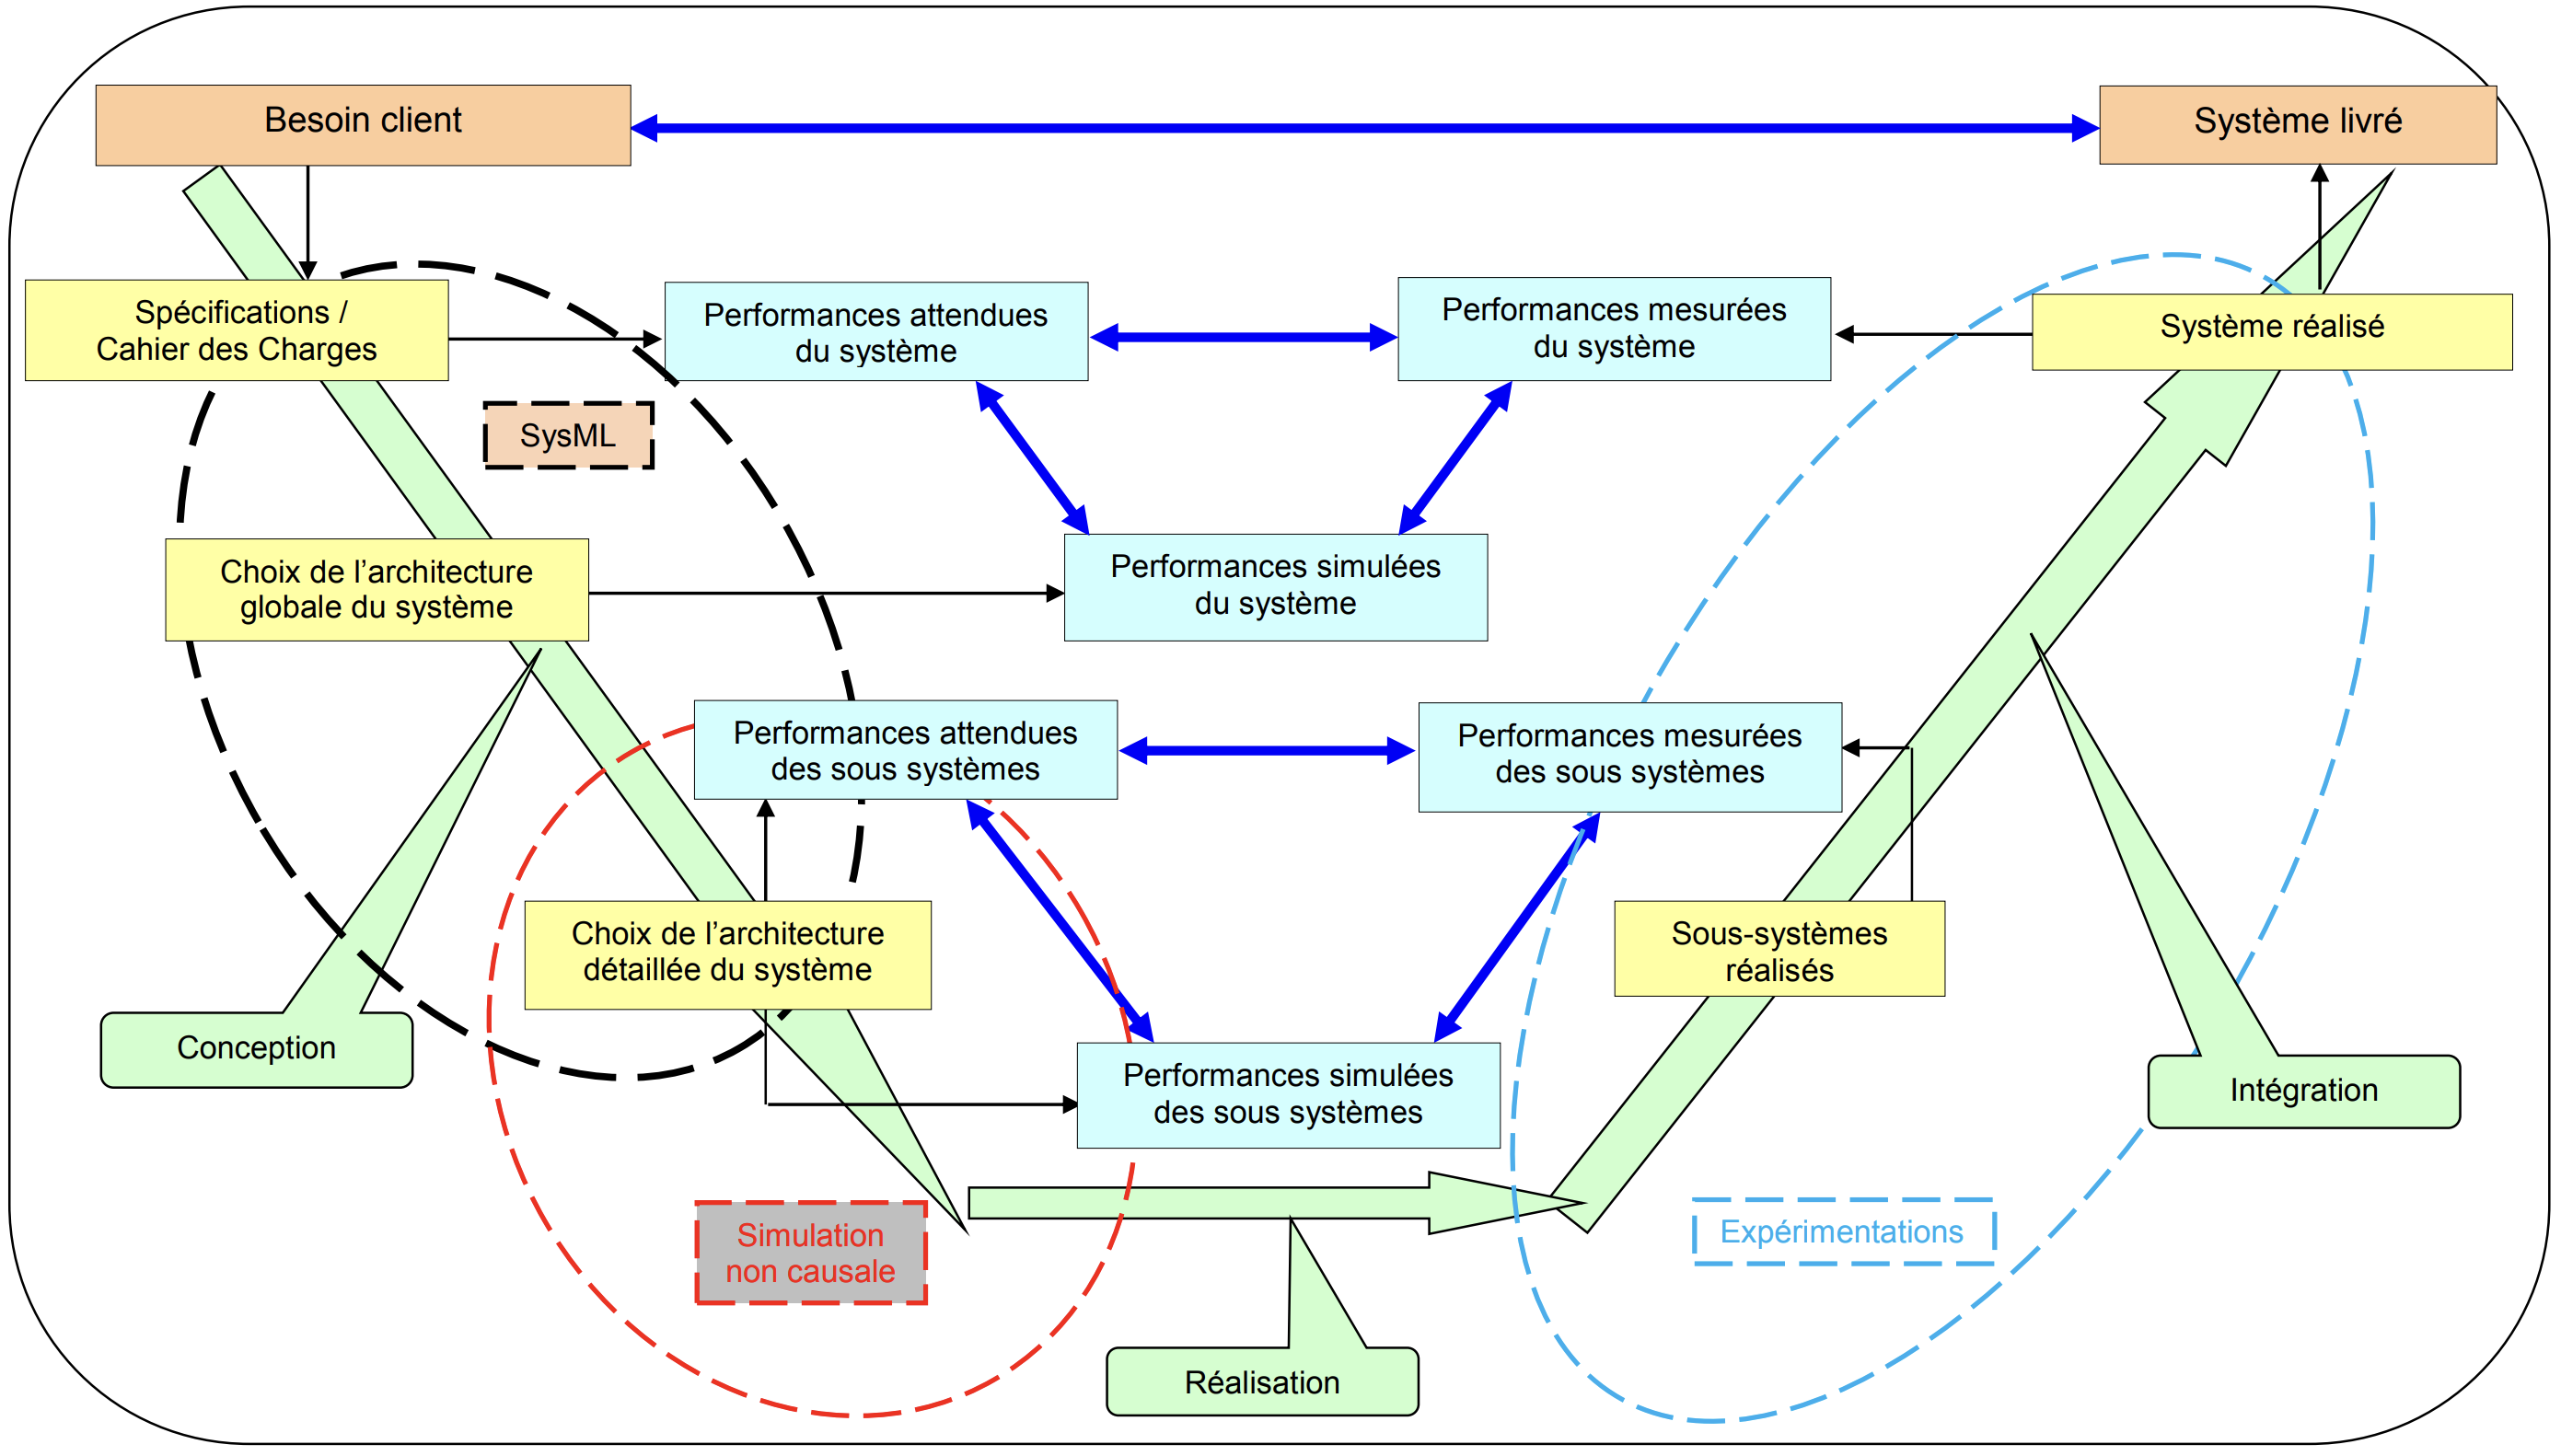
\includegraphics[width=0.8\textwidth,height=\textheight]{CM3/System-design.png}
\end{center}
\end{frame}

\subsection{Solides Indeformables}\label{solides-indeformables}

\begin{frame}{Solides Indeformables}
\begin{figure}

\begin{minipage}{0.70\linewidth}

\begin{tcolorbox}[enhanced jigsaw, colbacktitle=quarto-callout-note-color!10!white, bottomrule=.15mm, opacitybacktitle=0.6, leftrule=.75mm, colback=white, arc=.35mm, left=2mm, title=\textcolor{quarto-callout-note-color}{\faInfo}\hspace{0.5em}{Conséquence géométrique}, breakable, colframe=quarto-callout-note-color-frame, toprule=.15mm, coltitle=black, bottomtitle=1mm, opacityback=0, toptitle=1mm, titlerule=0mm, rightrule=.15mm]

La distance entre deux points quelconques d'un solide indéformable est
invariable dans un \textbf{Repère donneé}

\end{tcolorbox}

\end{minipage}%
%
\begin{minipage}{0.30\linewidth}

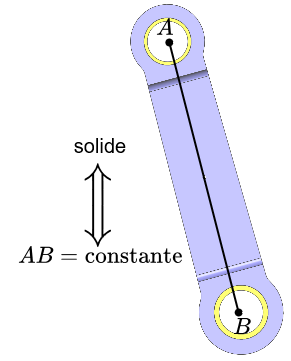
\includegraphics[width=0.9\textwidth,height=\textheight]{CM3/Solide-indeformable.png}

\subcaption{\label{}Bielle d'un micromoteur de modélisme}
\end{minipage}%

\end{figure}%
\end{frame}

\subsection{Repère}\label{repuxe8re}

\begin{frame}{Repère}
\begin{figure}

\begin{minipage}{0.60\linewidth}
Pour connaitre la position de tous ses points dans l'espace, il suffit
de connaitre la position d'un repère lié à ce solide. \textbf{Repère de
référence}: \(R(O, \vec{x}, \vec{y}, \vec{z})\) \textbf{Repère de lié au
solide.}: \(R(O_1, \vec{x_1}, \vec{y_1}, \vec{z_1})\)\end{minipage}%
%
\begin{minipage}{0.40\linewidth}
\begin{center}
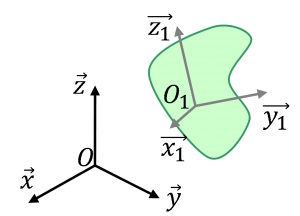
\includegraphics[width=0.8\textwidth,height=\textheight]{CM3/Repere.png}
\end{center}
\end{minipage}%

\end{figure}%

\pause

La position du solide dans l'espace, est déterminée par \emph{6
paramètres indépendants}

\begin{enumerate}
\tightlist
\item
  Position du point \(O_1\) → \textbf{3 Coordonnées}
\item
  Orientation de \(\vec{x_1}, \vec{y_1}, \vec{z_1})\) par rapport à
  \(R(O, \vec{x}, \vec{y}, \vec{z})\) → \textbf{3 Angles}
\end{enumerate}
\end{frame}

\begin{frame}{Repère}
\phantomsection\label{repuxe8re-1}
\emph{Exemple} : Repère local lié au Solide 2 (la bielle) et Repère de
référence, lié au solide 0 (le bâti)

\begin{figure}

\begin{minipage}{0.50\linewidth}
\begin{center}
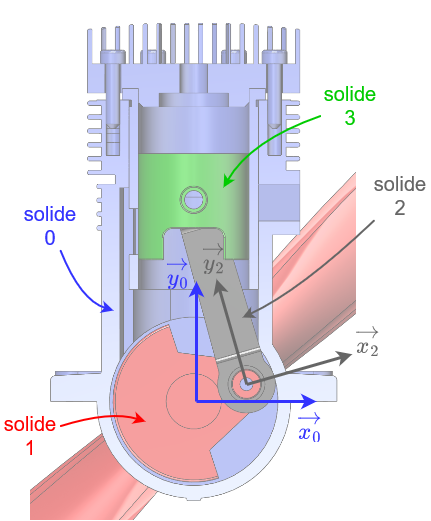
\includegraphics[width=0.7\textwidth,height=\textheight]{CM3/Repere-01.png}
\end{center}
\end{minipage}%
%
\begin{minipage}{0.50\linewidth}
\begin{center}
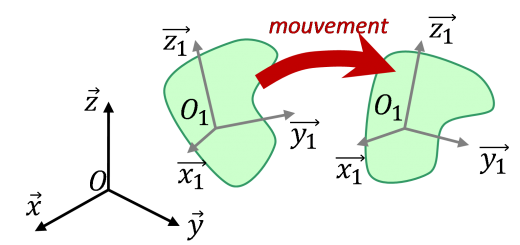
\includegraphics[width=0.7\textwidth,height=\textheight]{CM3/Repere-02.gif}
\end{center}
\end{minipage}%

\end{figure}%
\end{frame}

\subsection{Degree de liberté}\label{degree-de-libertuxe9}

\begin{frame}{Degree de liberté}
Il existe deux \emph{mouvements élémentaires} entre les solides :

\begin{figure}

\begin{minipage}{0.55\linewidth}

\begin{enumerate}
\tightlist
\item
  \textbf{TRANSLATION (RECTILIGNE)} : les trajectoires de tous les
  points du solide sont des droites parallèles.
\item
  \textbf{ROTATION} : les trajectoires de chaque point sont des cercles
  coaxiaux.
\end{enumerate}

\end{minipage}%
%
\begin{minipage}{0.46\linewidth}
\begin{center}
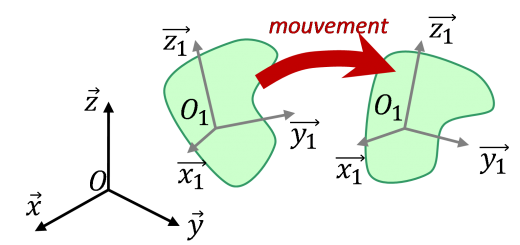
\includegraphics[width=1\textwidth,height=\textheight]{CM3/Repere-02.png}
\end{center}
\end{minipage}%

\end{figure}%

On appelle \emph{libertés} d'un solide par rapport à un référentiel, les
mouvements indépendants de ce solide pour passer d'une position à une
autre.
\end{frame}

\begin{frame}{Degree de Liberté}
\phantomsection\label{degree-de-libertuxe9-1}
\begin{enumerate}
\tightlist
\item
  \textbf{TRANSLATION (RECTILIGNE)} : les trajectoires de tous les
  points du solide sont des droites parallèles.

  \begin{itemize}
  \tightlist
  \item
    \(T_x, T_y, T_z\) selon \((x,y,z)\)
  \end{itemize}
\item
  \textbf{ROTATION} : les trajectoires de chaque point sont des cercles
  coaxiaux.

  \begin{itemize}
  \tightlist
  \item
    \(R_x, R_y, R_z\) autour des axes \((x,y,z)\)
  \end{itemize}
\end{enumerate}

\textbf{6 Degrees de liberté}
\end{frame}

\subsection{Notion de liaison}\label{notion-de-liaison}

\begin{frame}{Notion de liaison}
On appelle \textbf{liaison} entre deux solides l'ensemble des couples de
surfaces en contact entre ces deux solides, \textbf{visant à diminuer la
mobilité entre ces deux solides}.

\textbf{Zones de Contacts}

\begin{center}
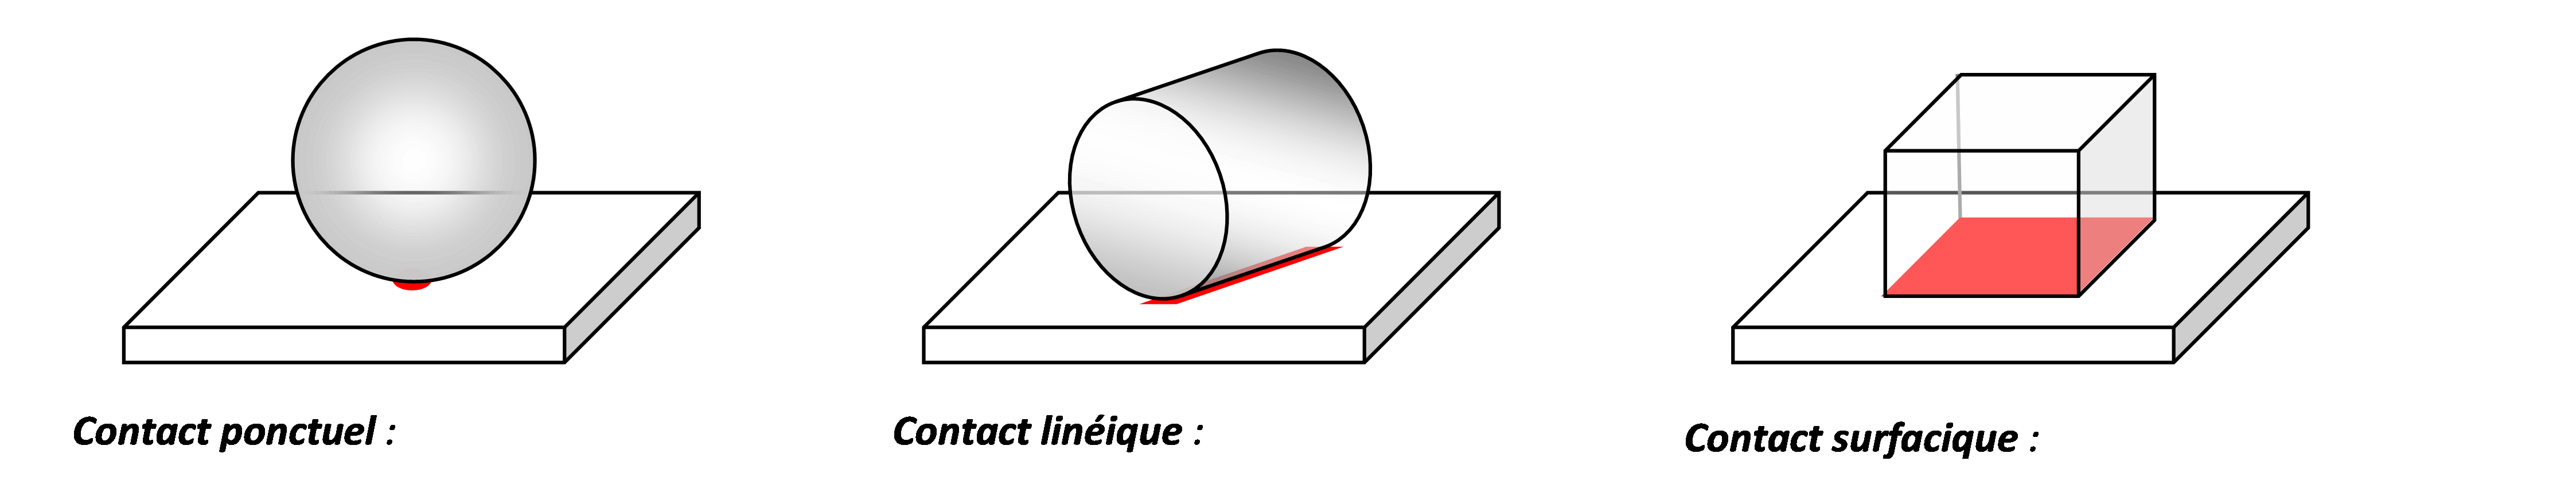
\includegraphics[width=0.8\textwidth,height=\textheight]{CM3/Contact.png}
\end{center}
\end{frame}

\subsection{Degrés de liberté d'une
liaison}\label{degruxe9s-de-libertuxe9-dune-liaison}

\begin{frame}{Degrés de liberté d'une liaison}
Les \emph{degrés de liberté d'une liaison} sont \textbf{les déplacements
élémentaires indépendants} autorisés par cette liaison.
\end{frame}

\subsection{Les Liaisons Mécaniques
Elementaires}\label{les-liaisons-muxe9caniques-elementaires}

\begin{frame}{Les Liaisons Mécaniques Elementaires}
Selon la norme NF EN ISO 3952-1
\end{frame}

\begin{frame}{Encastrement}
\phantomsection\label{encastrement}
\begin{center}
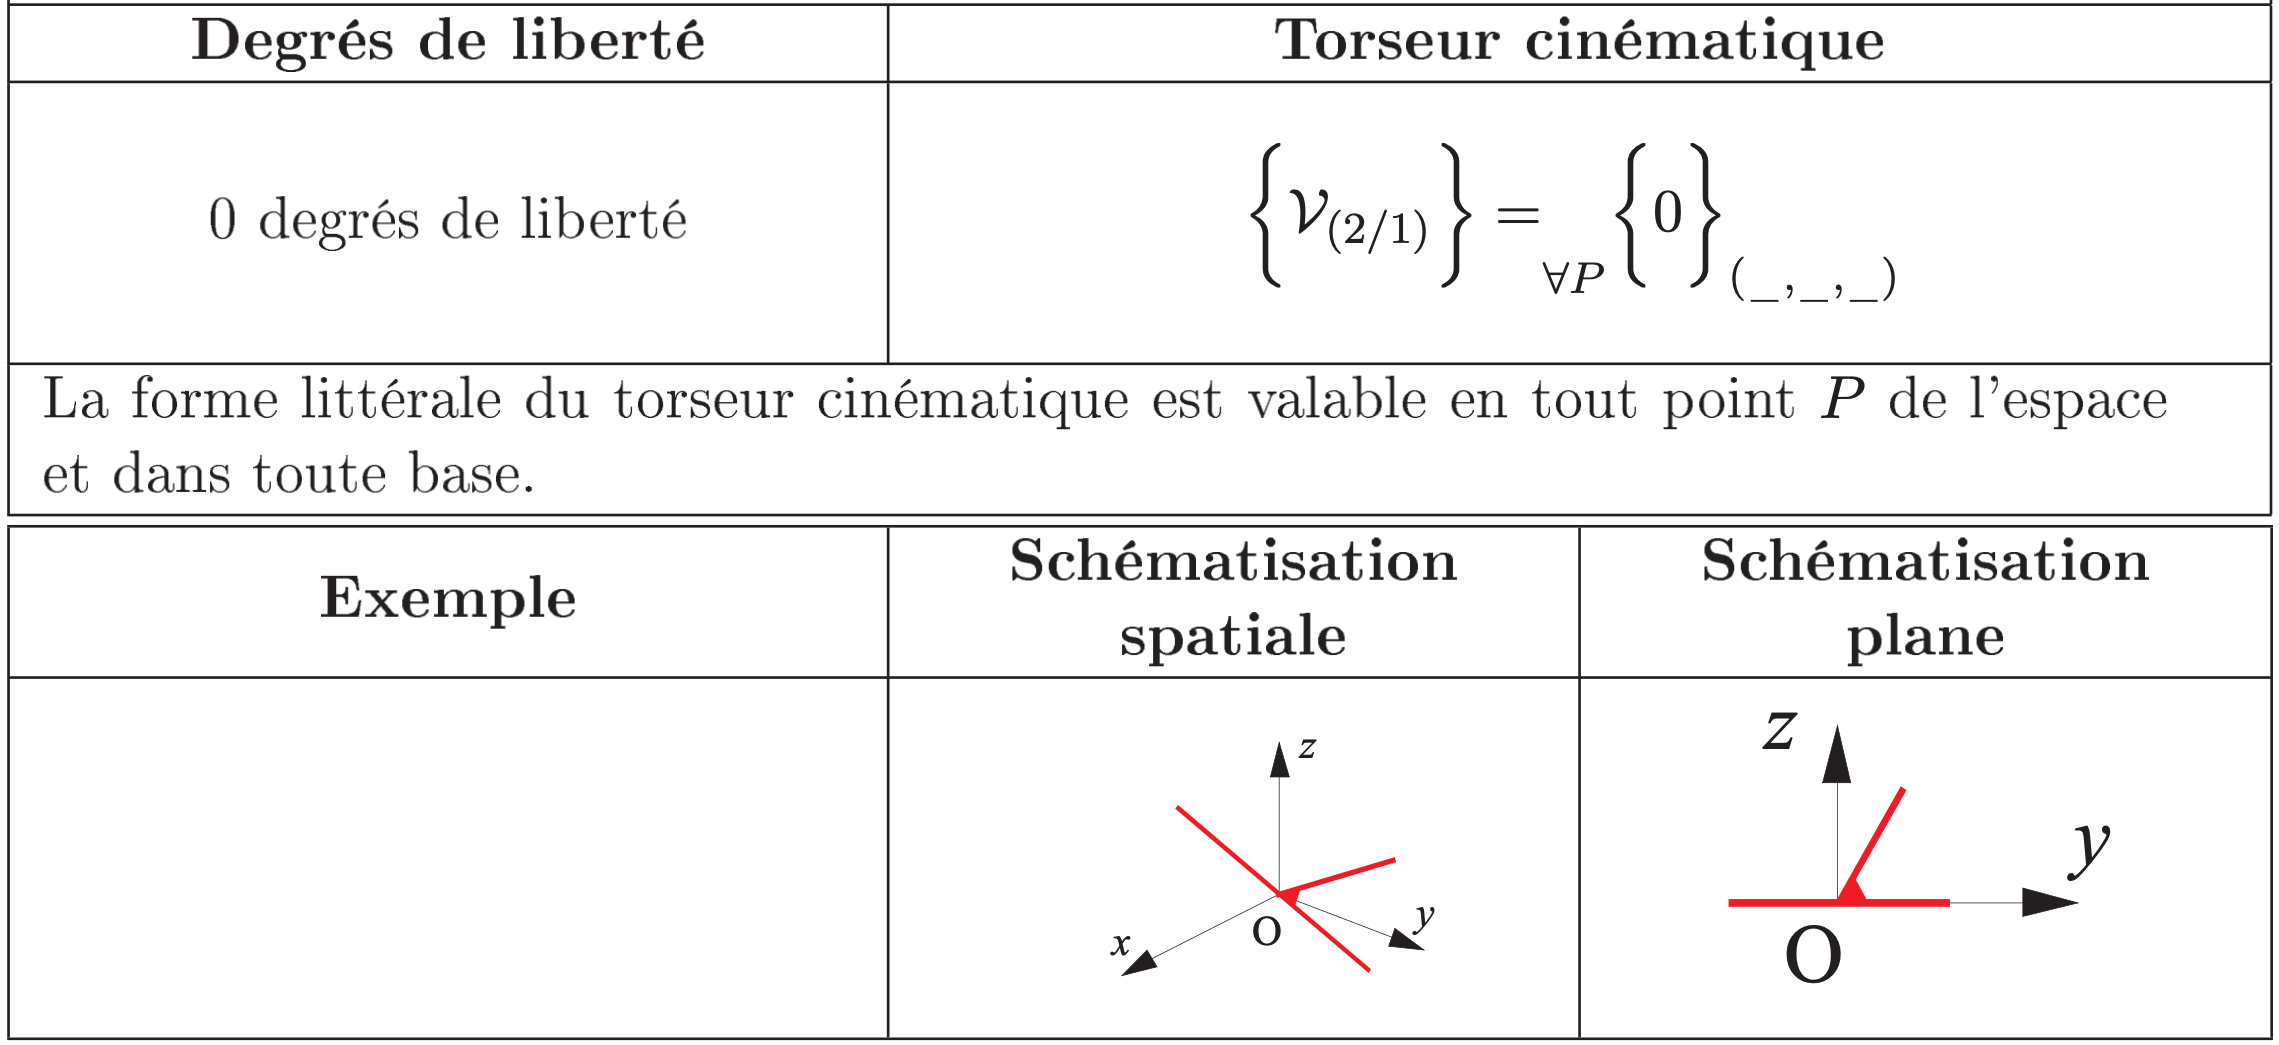
\includegraphics[width=0.8\textwidth,height=\textheight]{CM3/Liaison-Encastrement.png}
\end{center}
\end{frame}

\begin{frame}{Pivot d'Axe}
\phantomsection\label{pivot-daxe}
\begin{center}
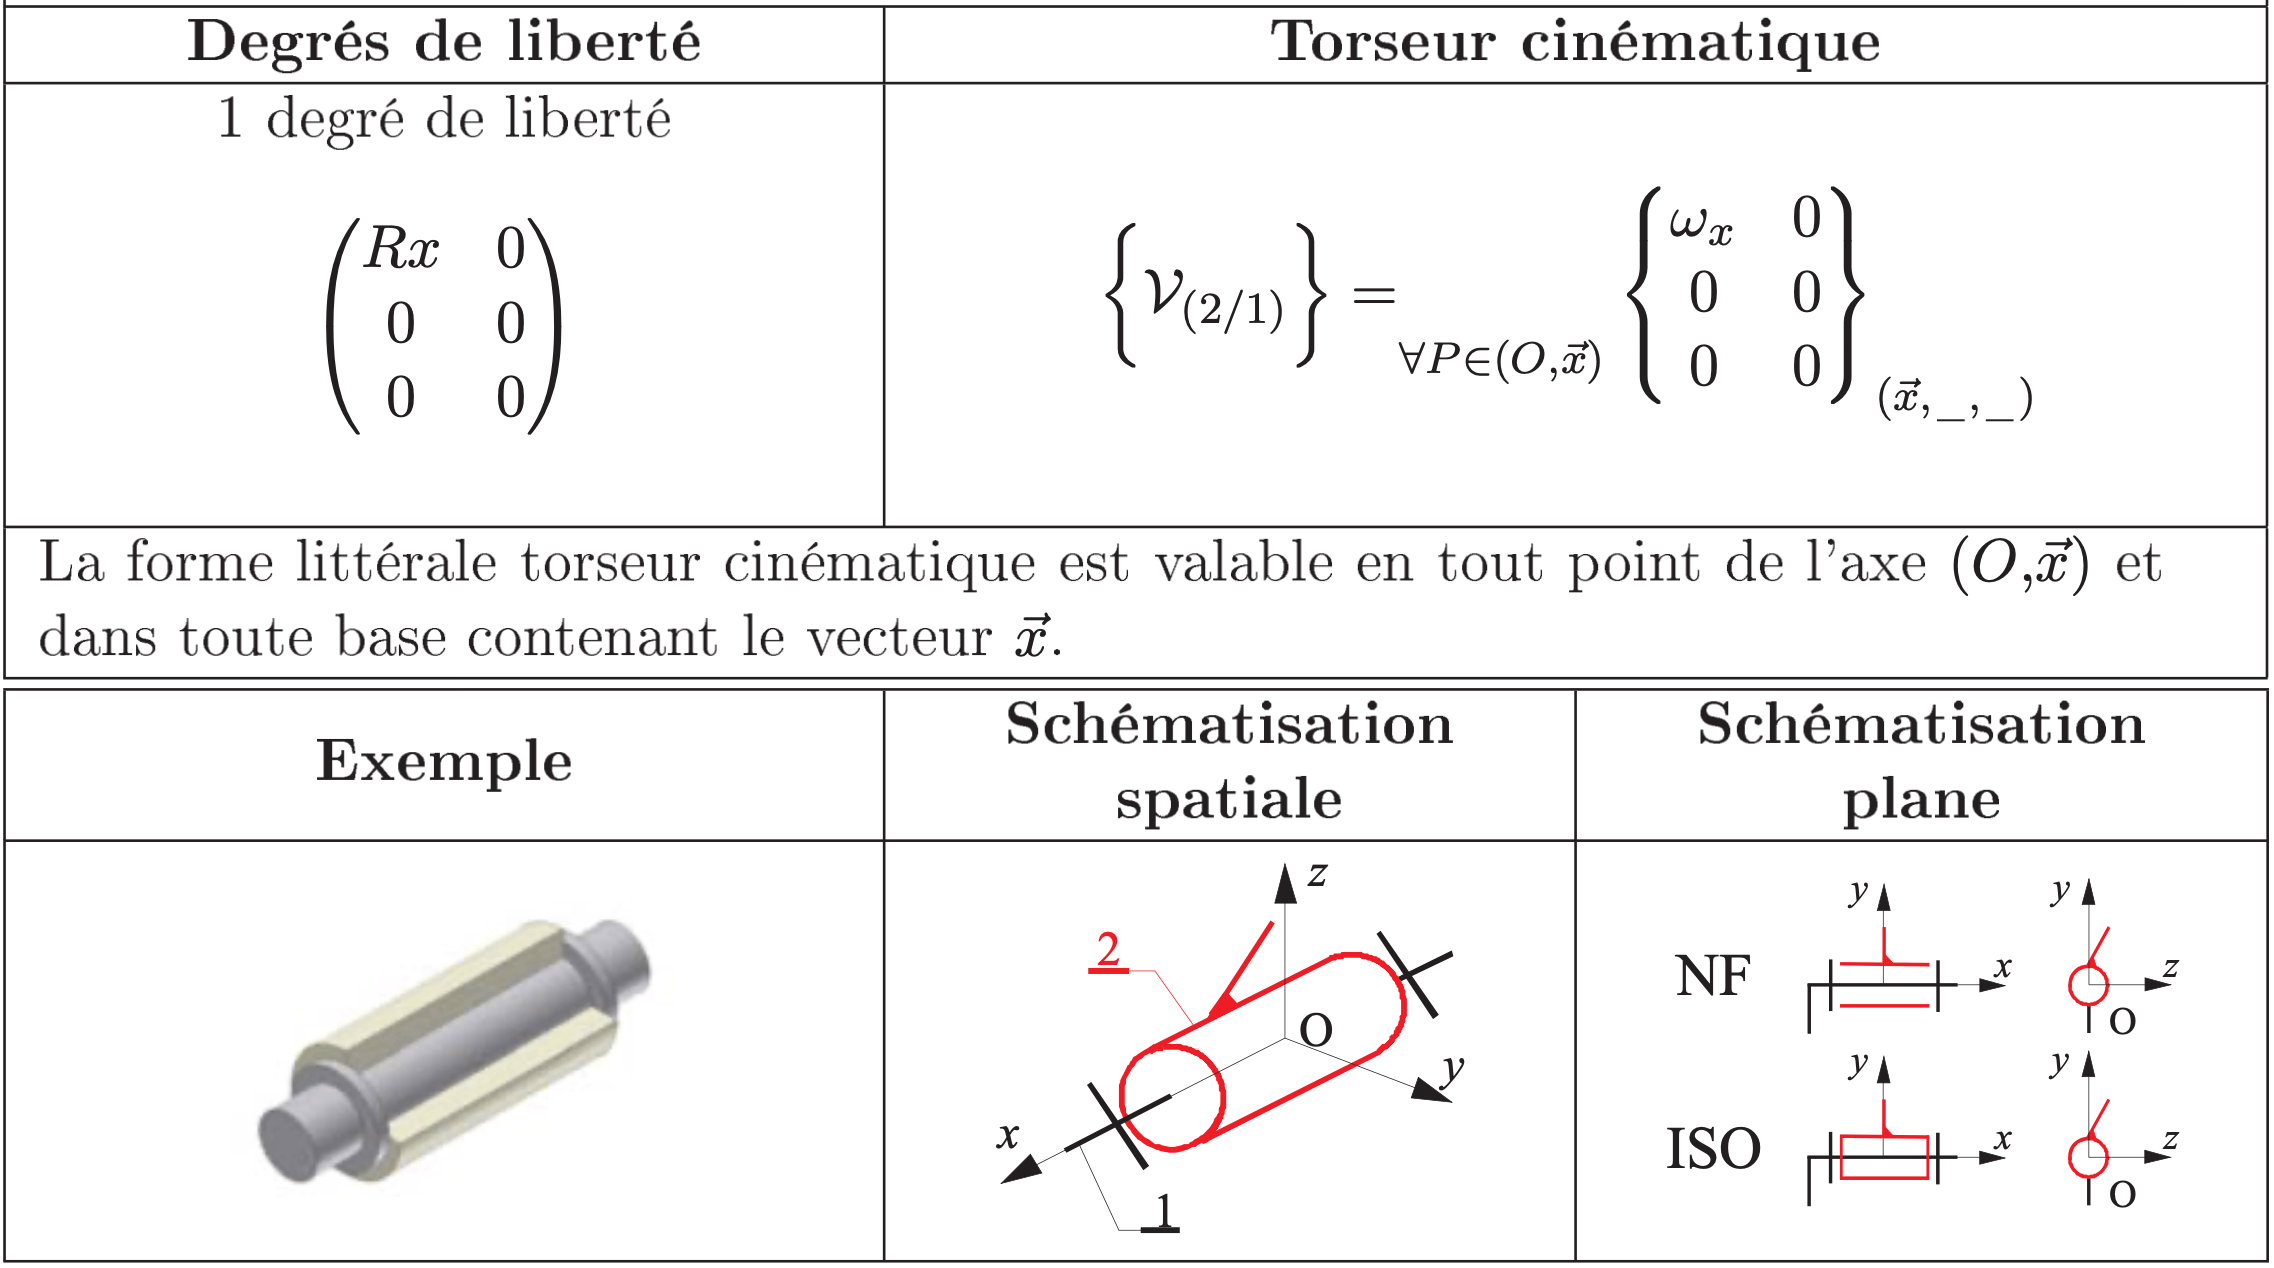
\includegraphics[width=0.8\textwidth,height=\textheight]{CM3/Liaison-Pivot.png}
\end{center}
\end{frame}

\begin{frame}{Glissière}
\phantomsection\label{glissiuxe8re}
\begin{center}
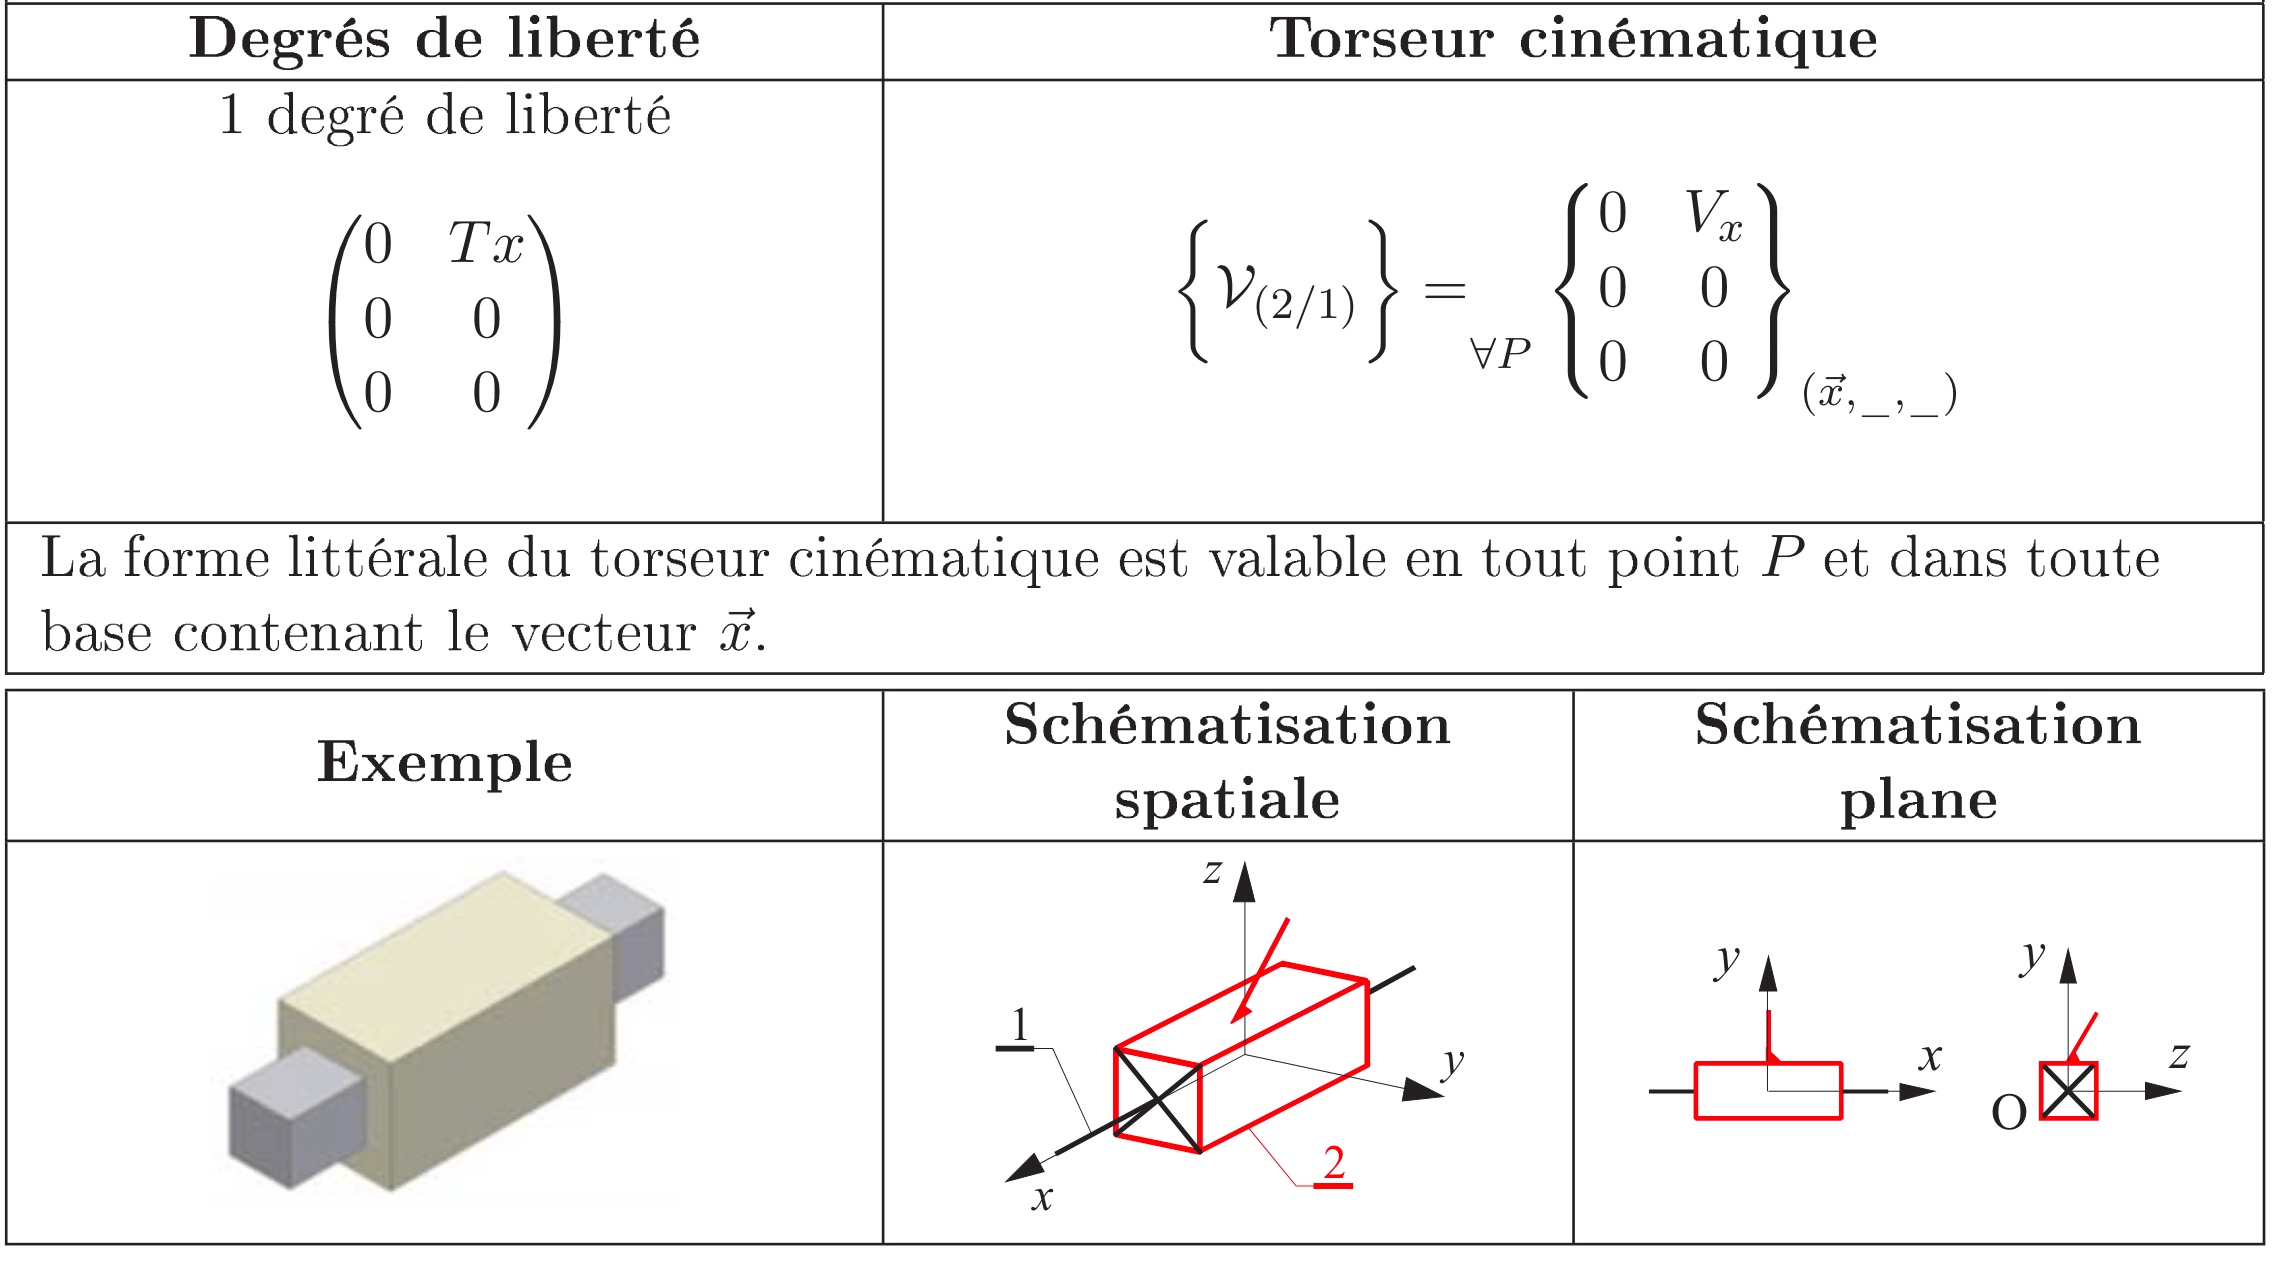
\includegraphics[width=0.8\textwidth,height=\textheight]{CM3/Liaison-Glissiere.pdf}
\end{center}
\end{frame}

\begin{frame}{Rotule}
\phantomsection\label{rotule}
\begin{block}{À vous !}
\begin{center}
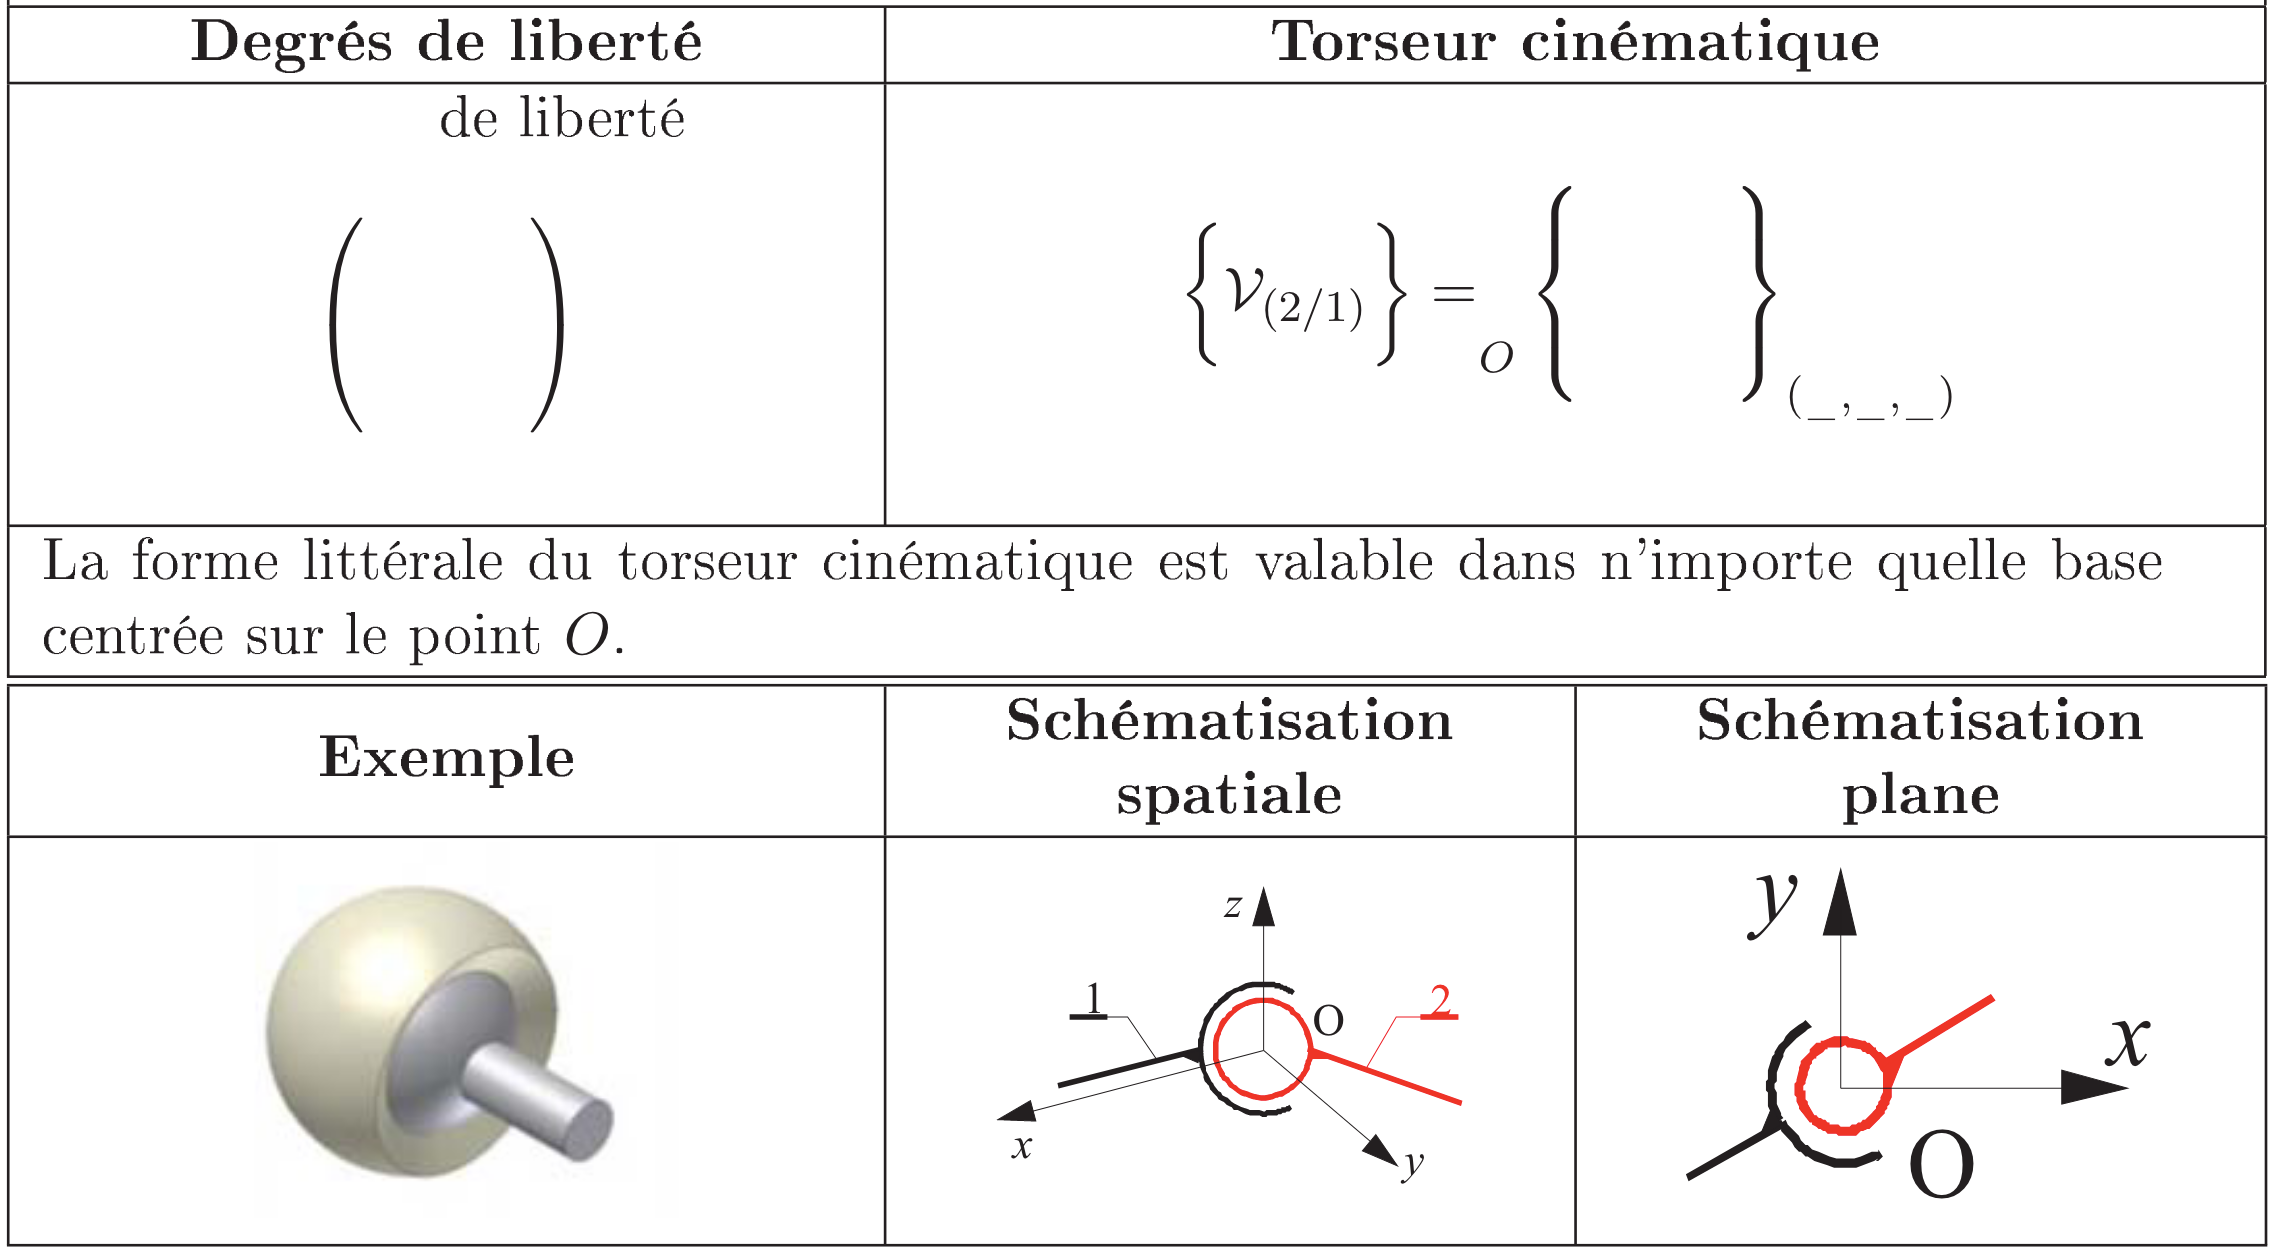
\includegraphics[width=0.7\textwidth,height=\textheight]{CM3/Liaison-rotule-00.png}
\end{center}
\end{block}

\begin{block}{Solution}
\begin{center}
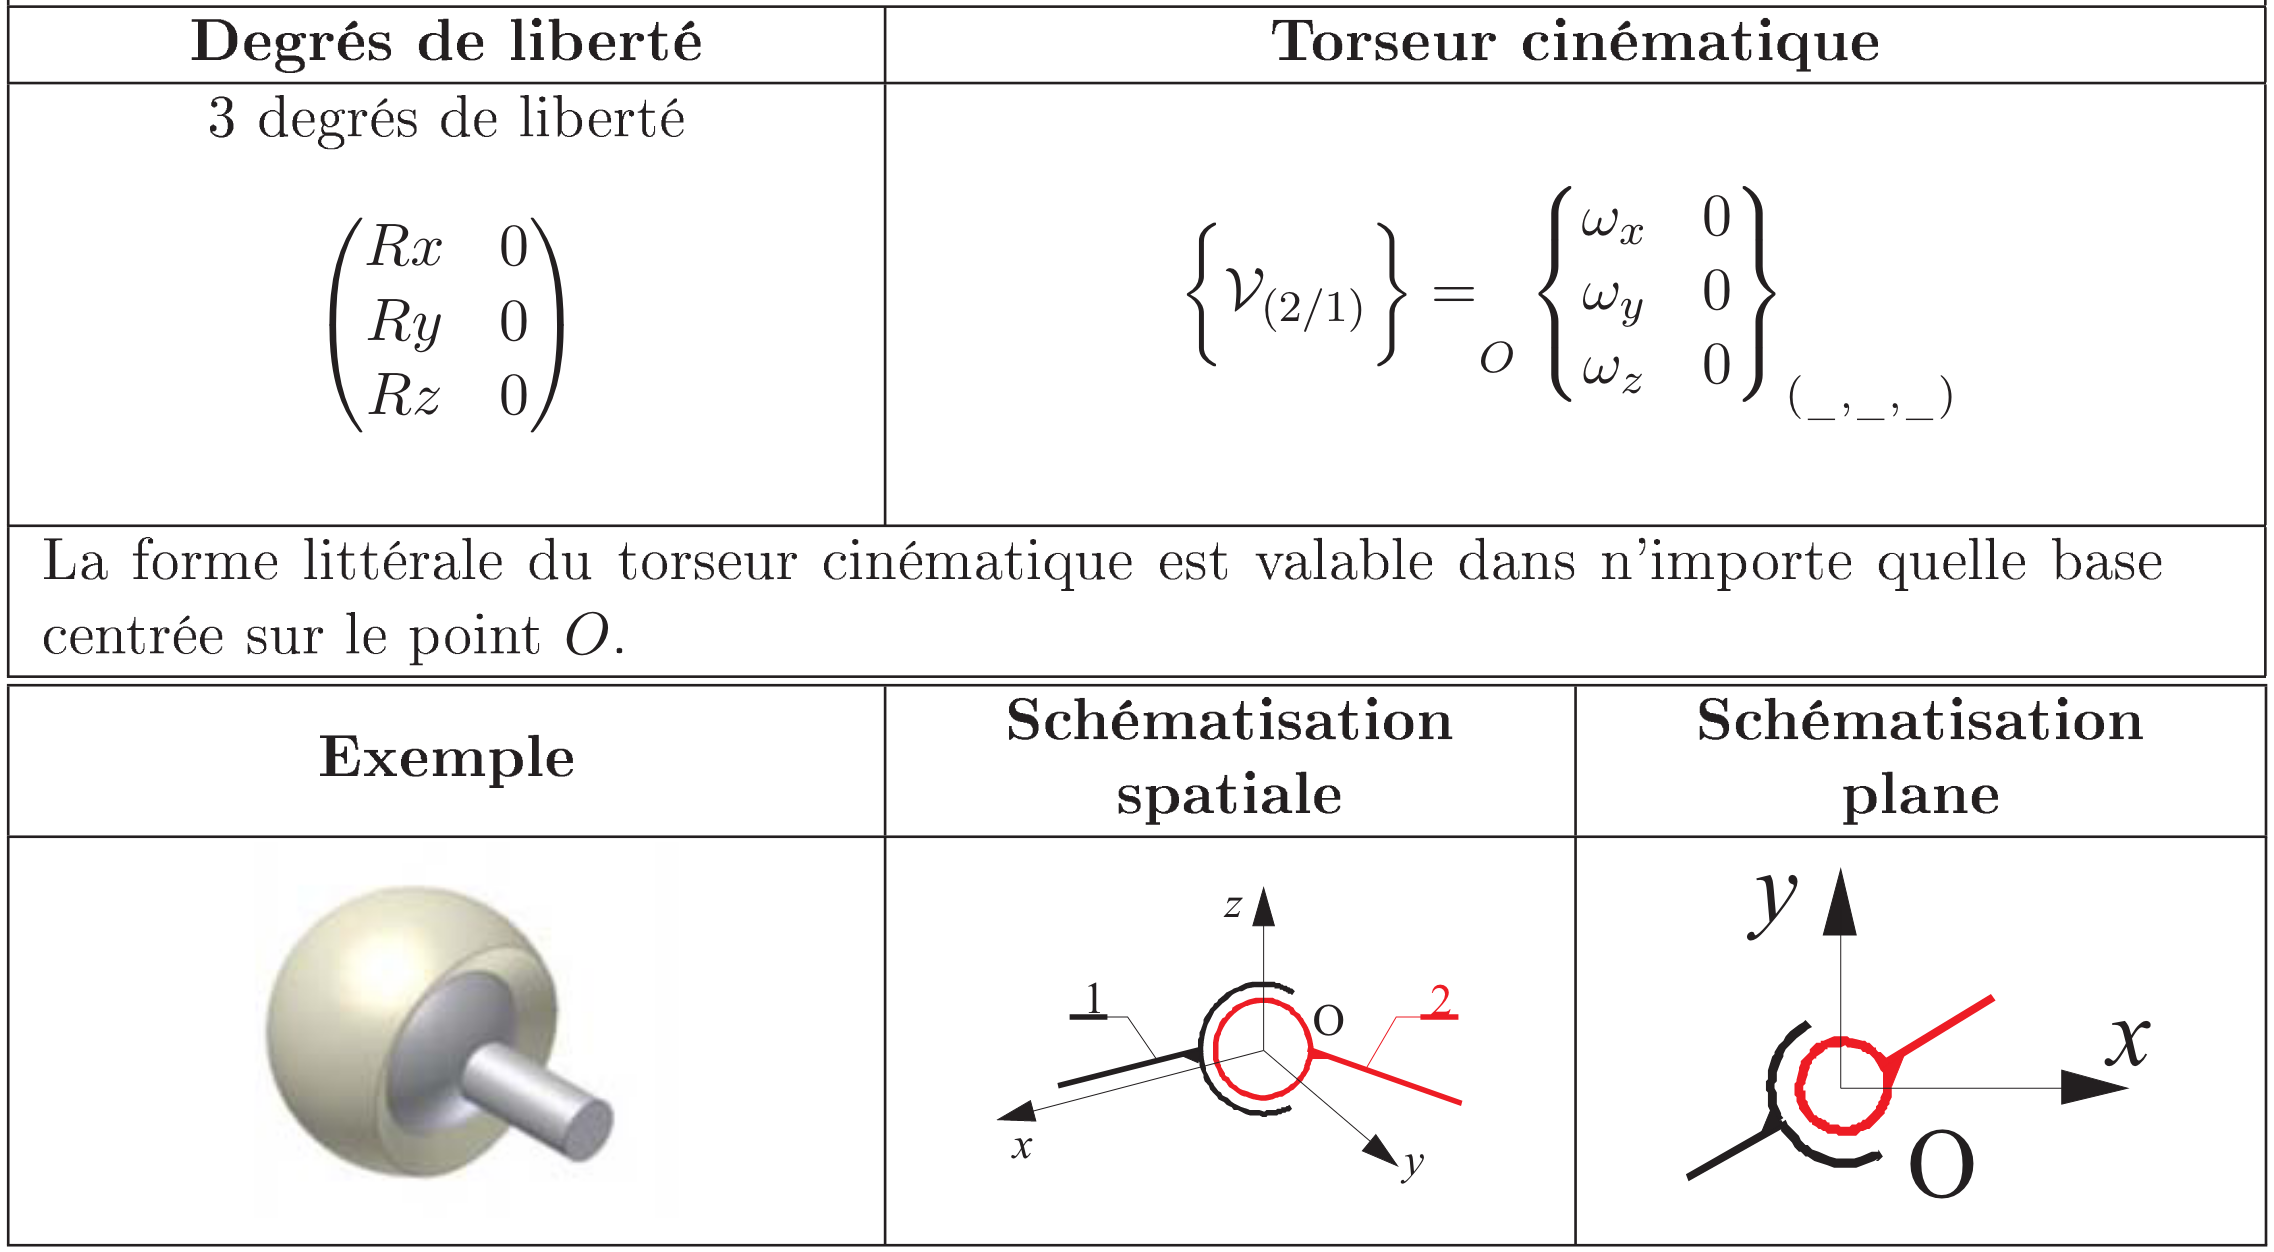
\includegraphics[width=0.7\textwidth,height=\textheight]{CM3/Liaison-rotule-01.png}
\end{center}
\end{block}
\end{frame}

\begin{frame}{Pivot glissant}
\phantomsection\label{pivot-glissant}
\begin{block}{À vous !}
\begin{center}
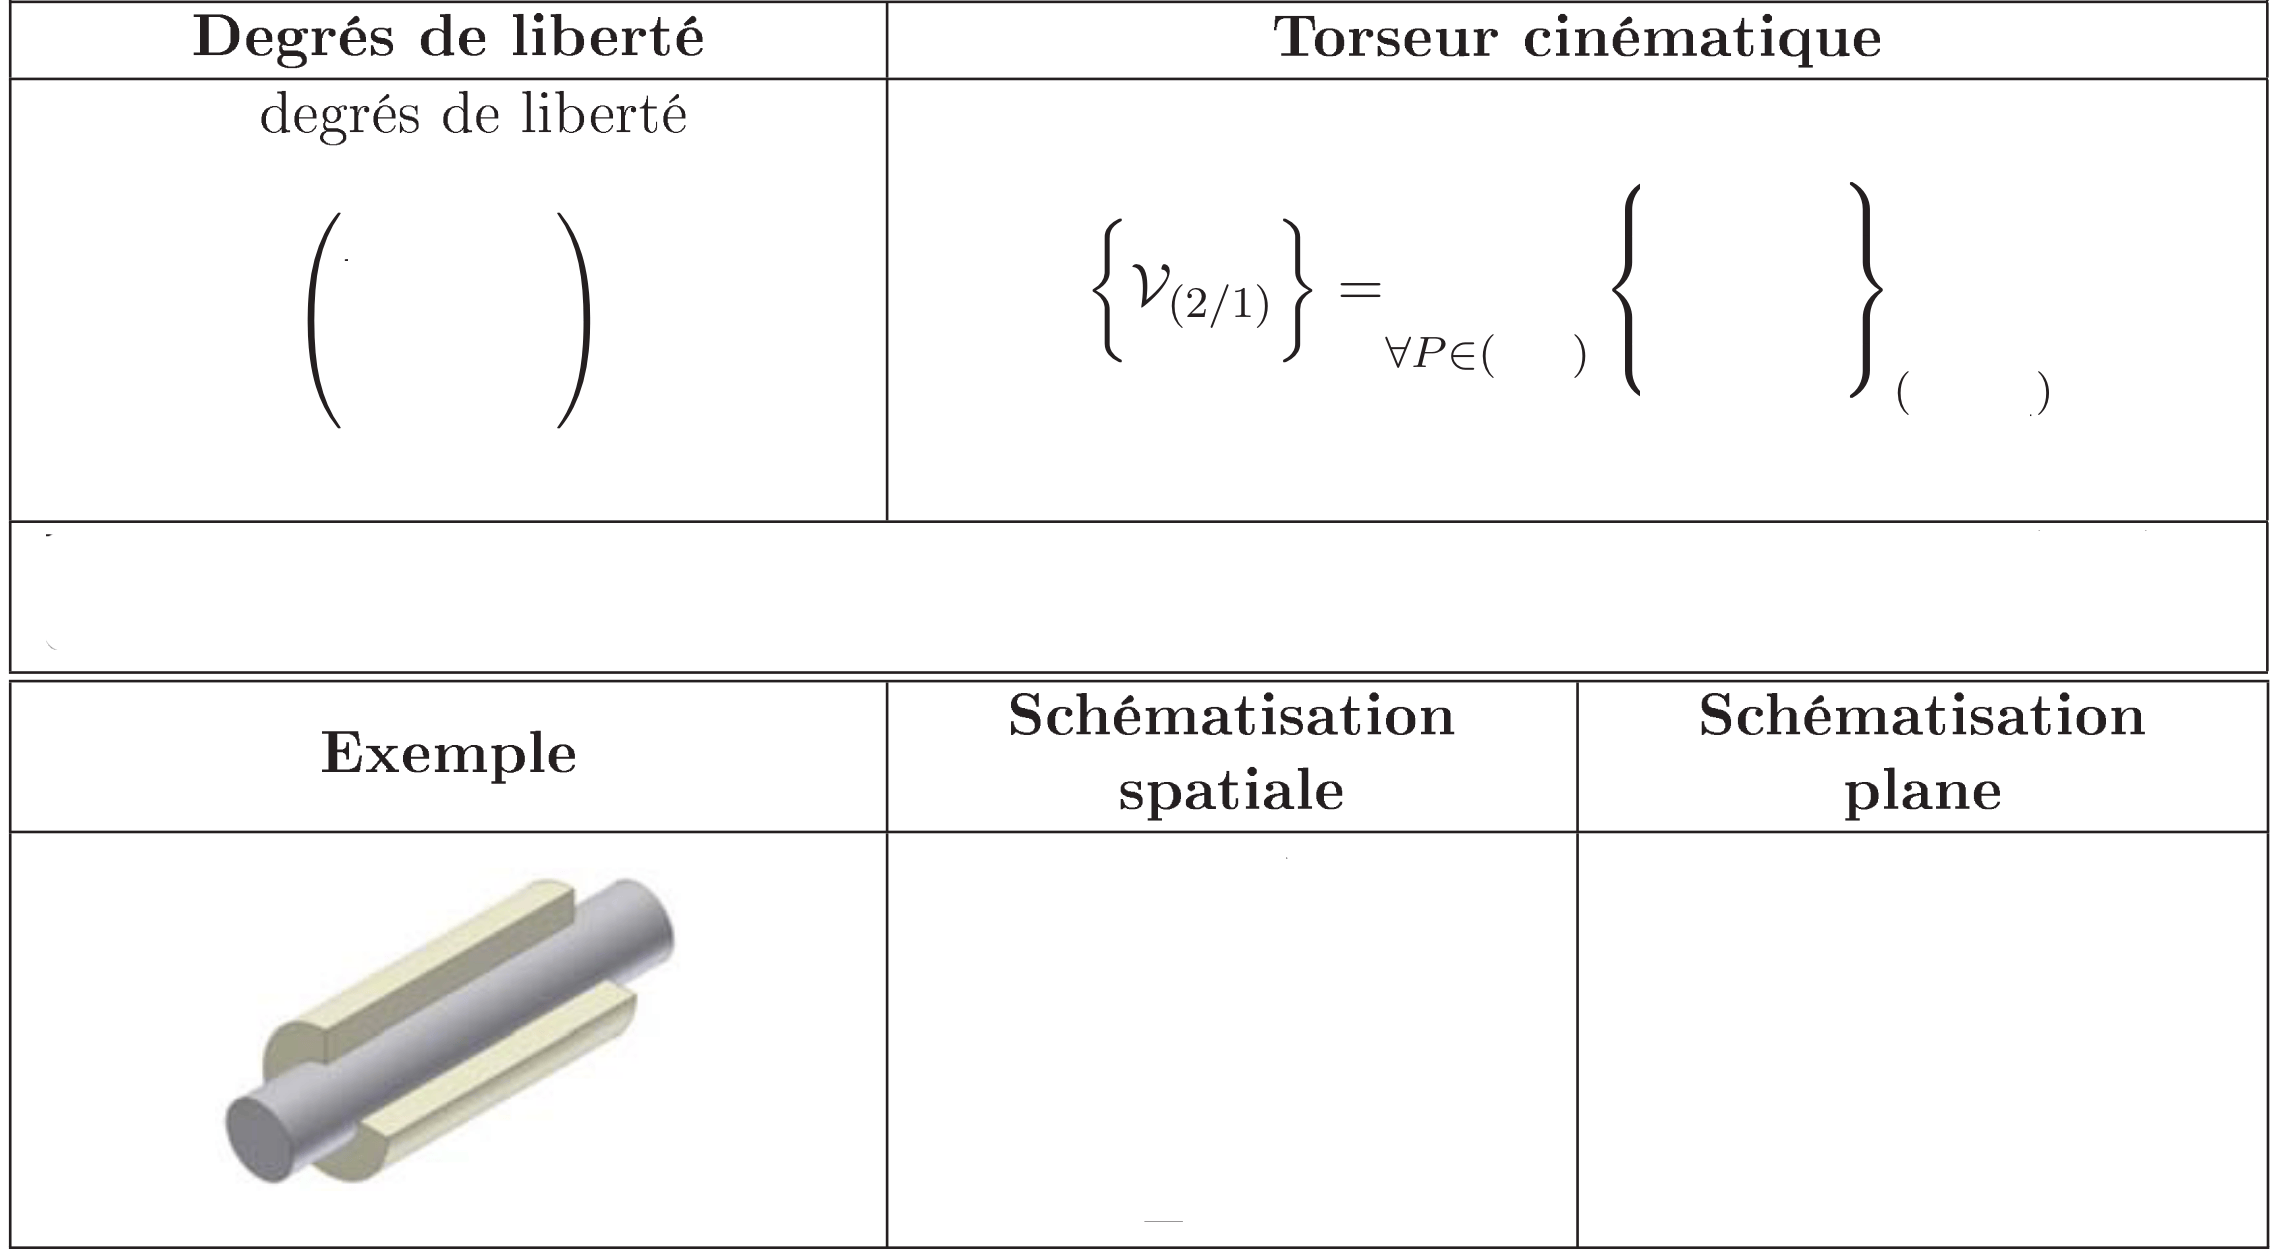
\includegraphics[width=0.7\textwidth,height=\textheight]{CM3/Liaison-Pivot-glissant-00.png}
\end{center}
\end{block}

\begin{block}{Solution}
\begin{center}
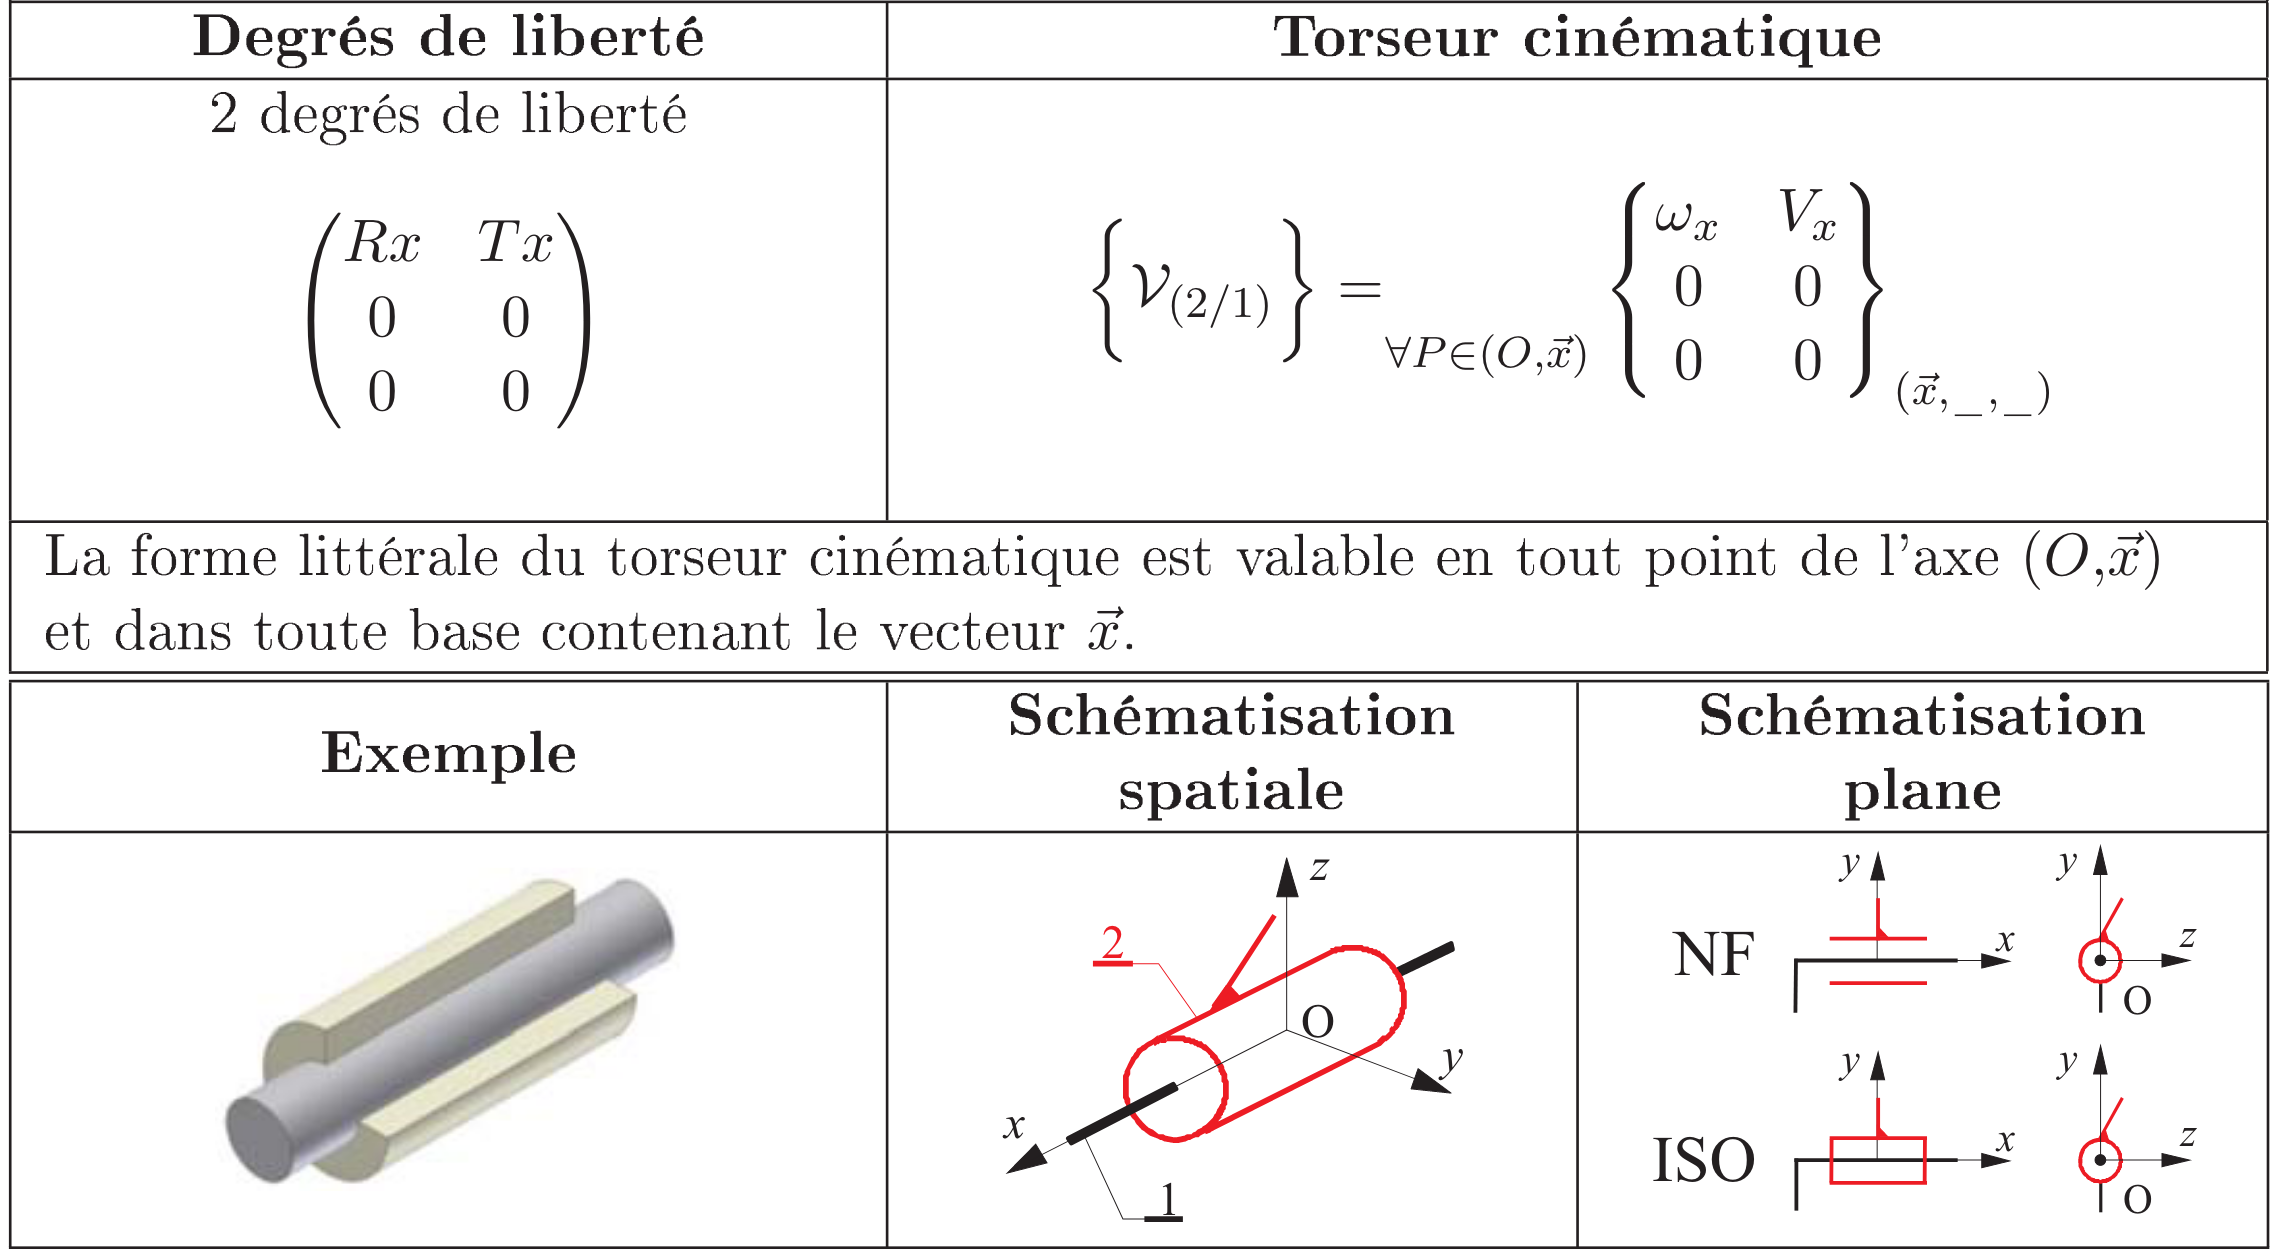
\includegraphics[width=0.7\textwidth,height=\textheight]{CM3/Liaison-Pivot-glissant-01.png}
\end{center}
\end{block}
\end{frame}

\begin{frame}{Appui Plan Normale}
\phantomsection\label{appui-plan-normale}
\begin{block}{À vous !}
\begin{center}
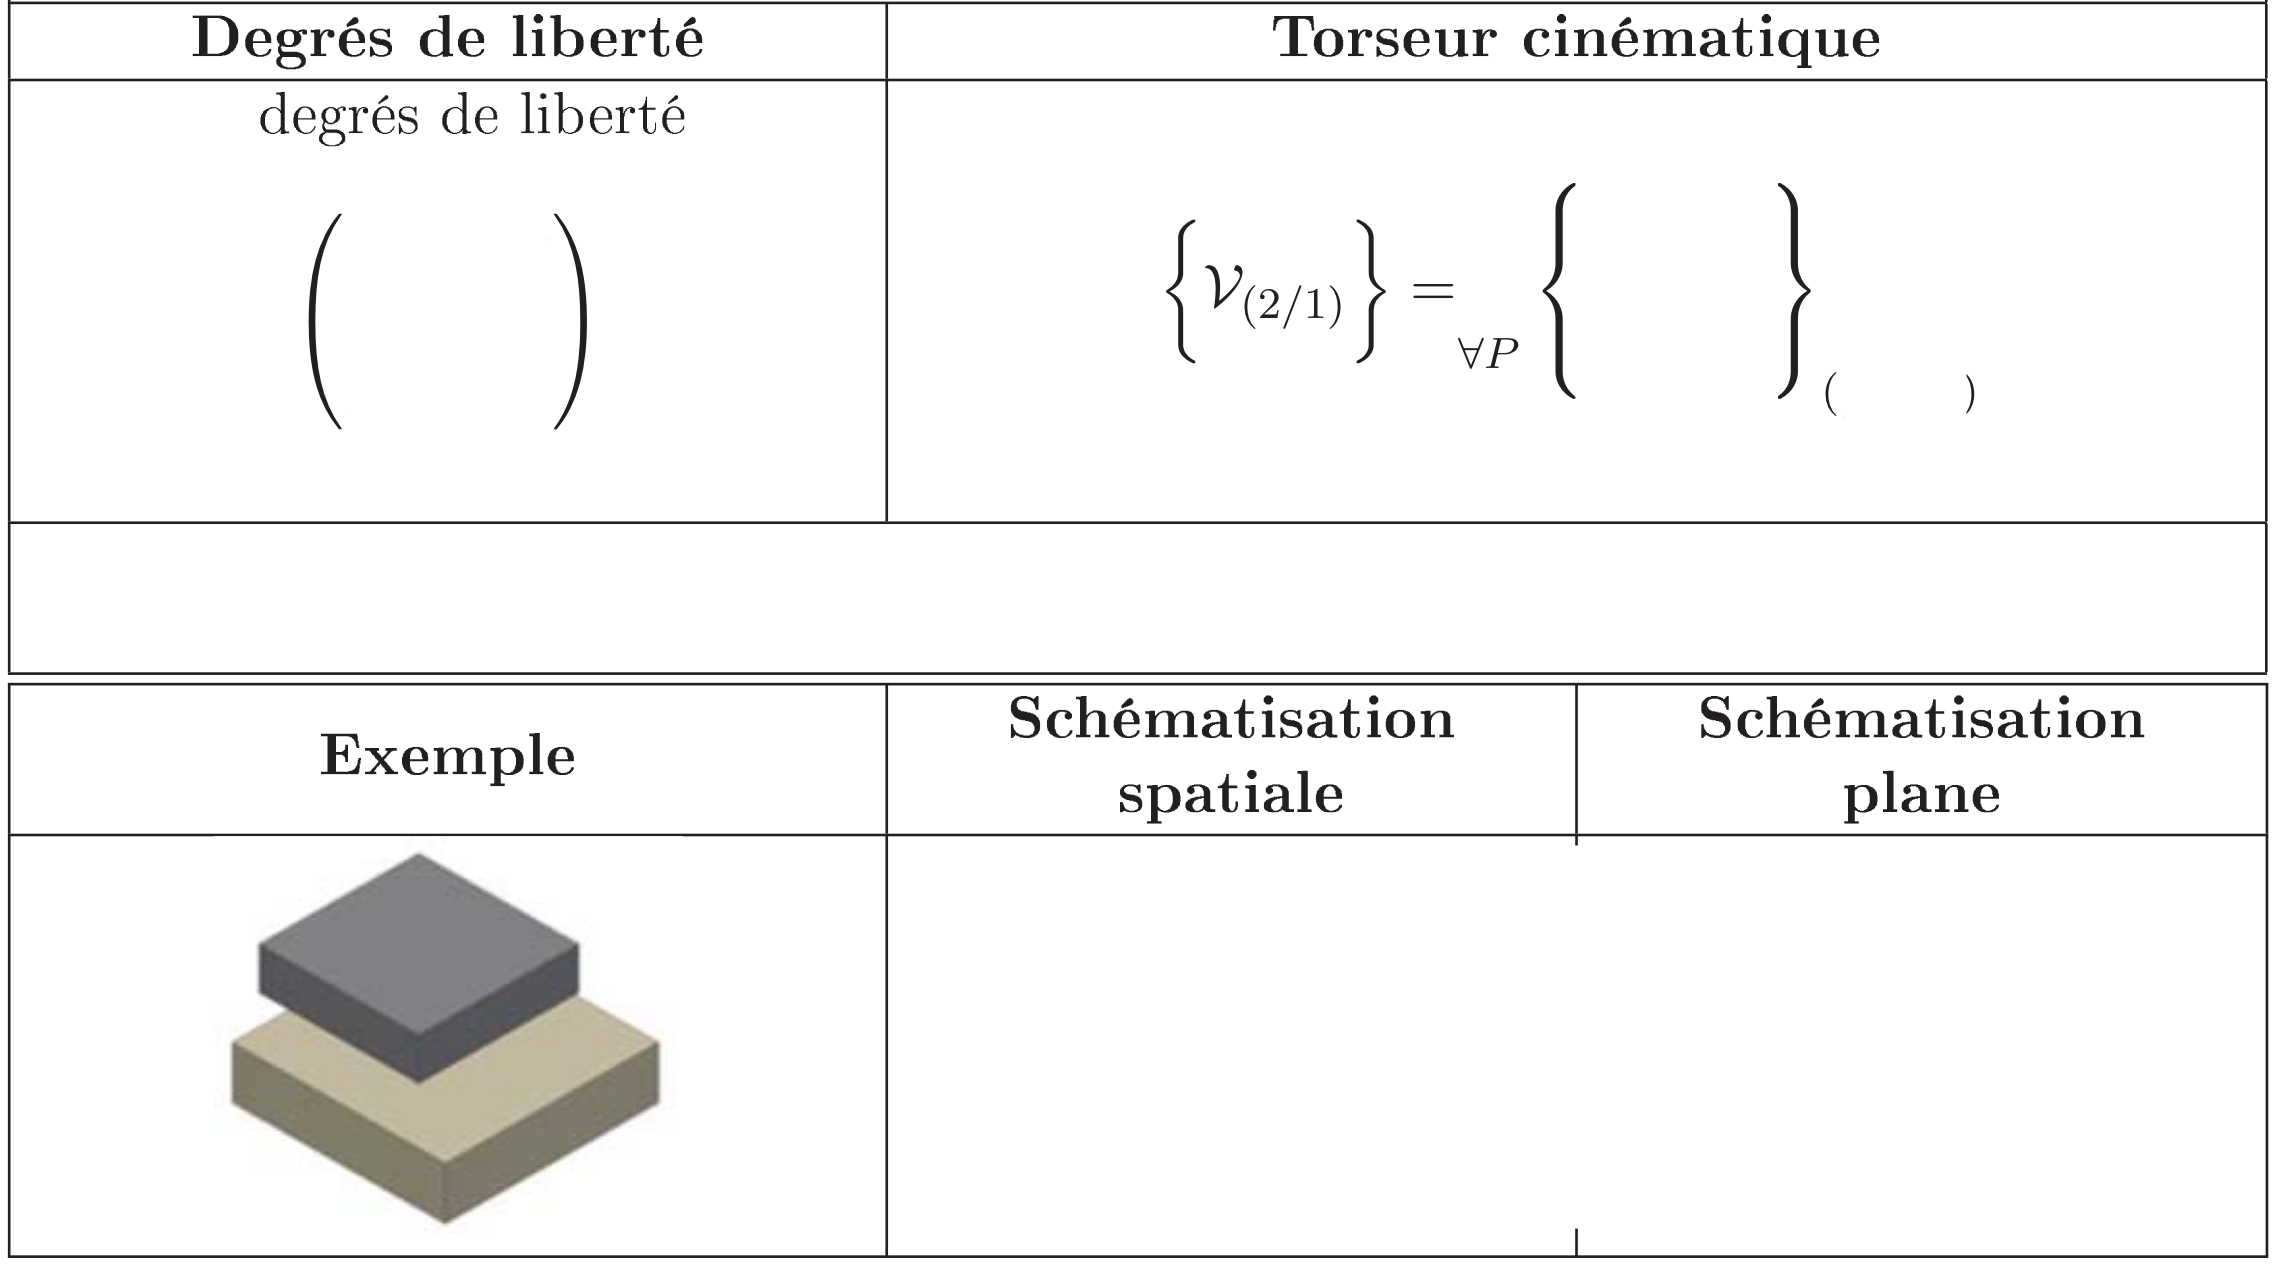
\includegraphics[width=0.7\textwidth,height=\textheight]{CM3/Liaison-Plan-00.png}
\end{center}
\end{block}

\begin{block}{Solution}
\begin{center}
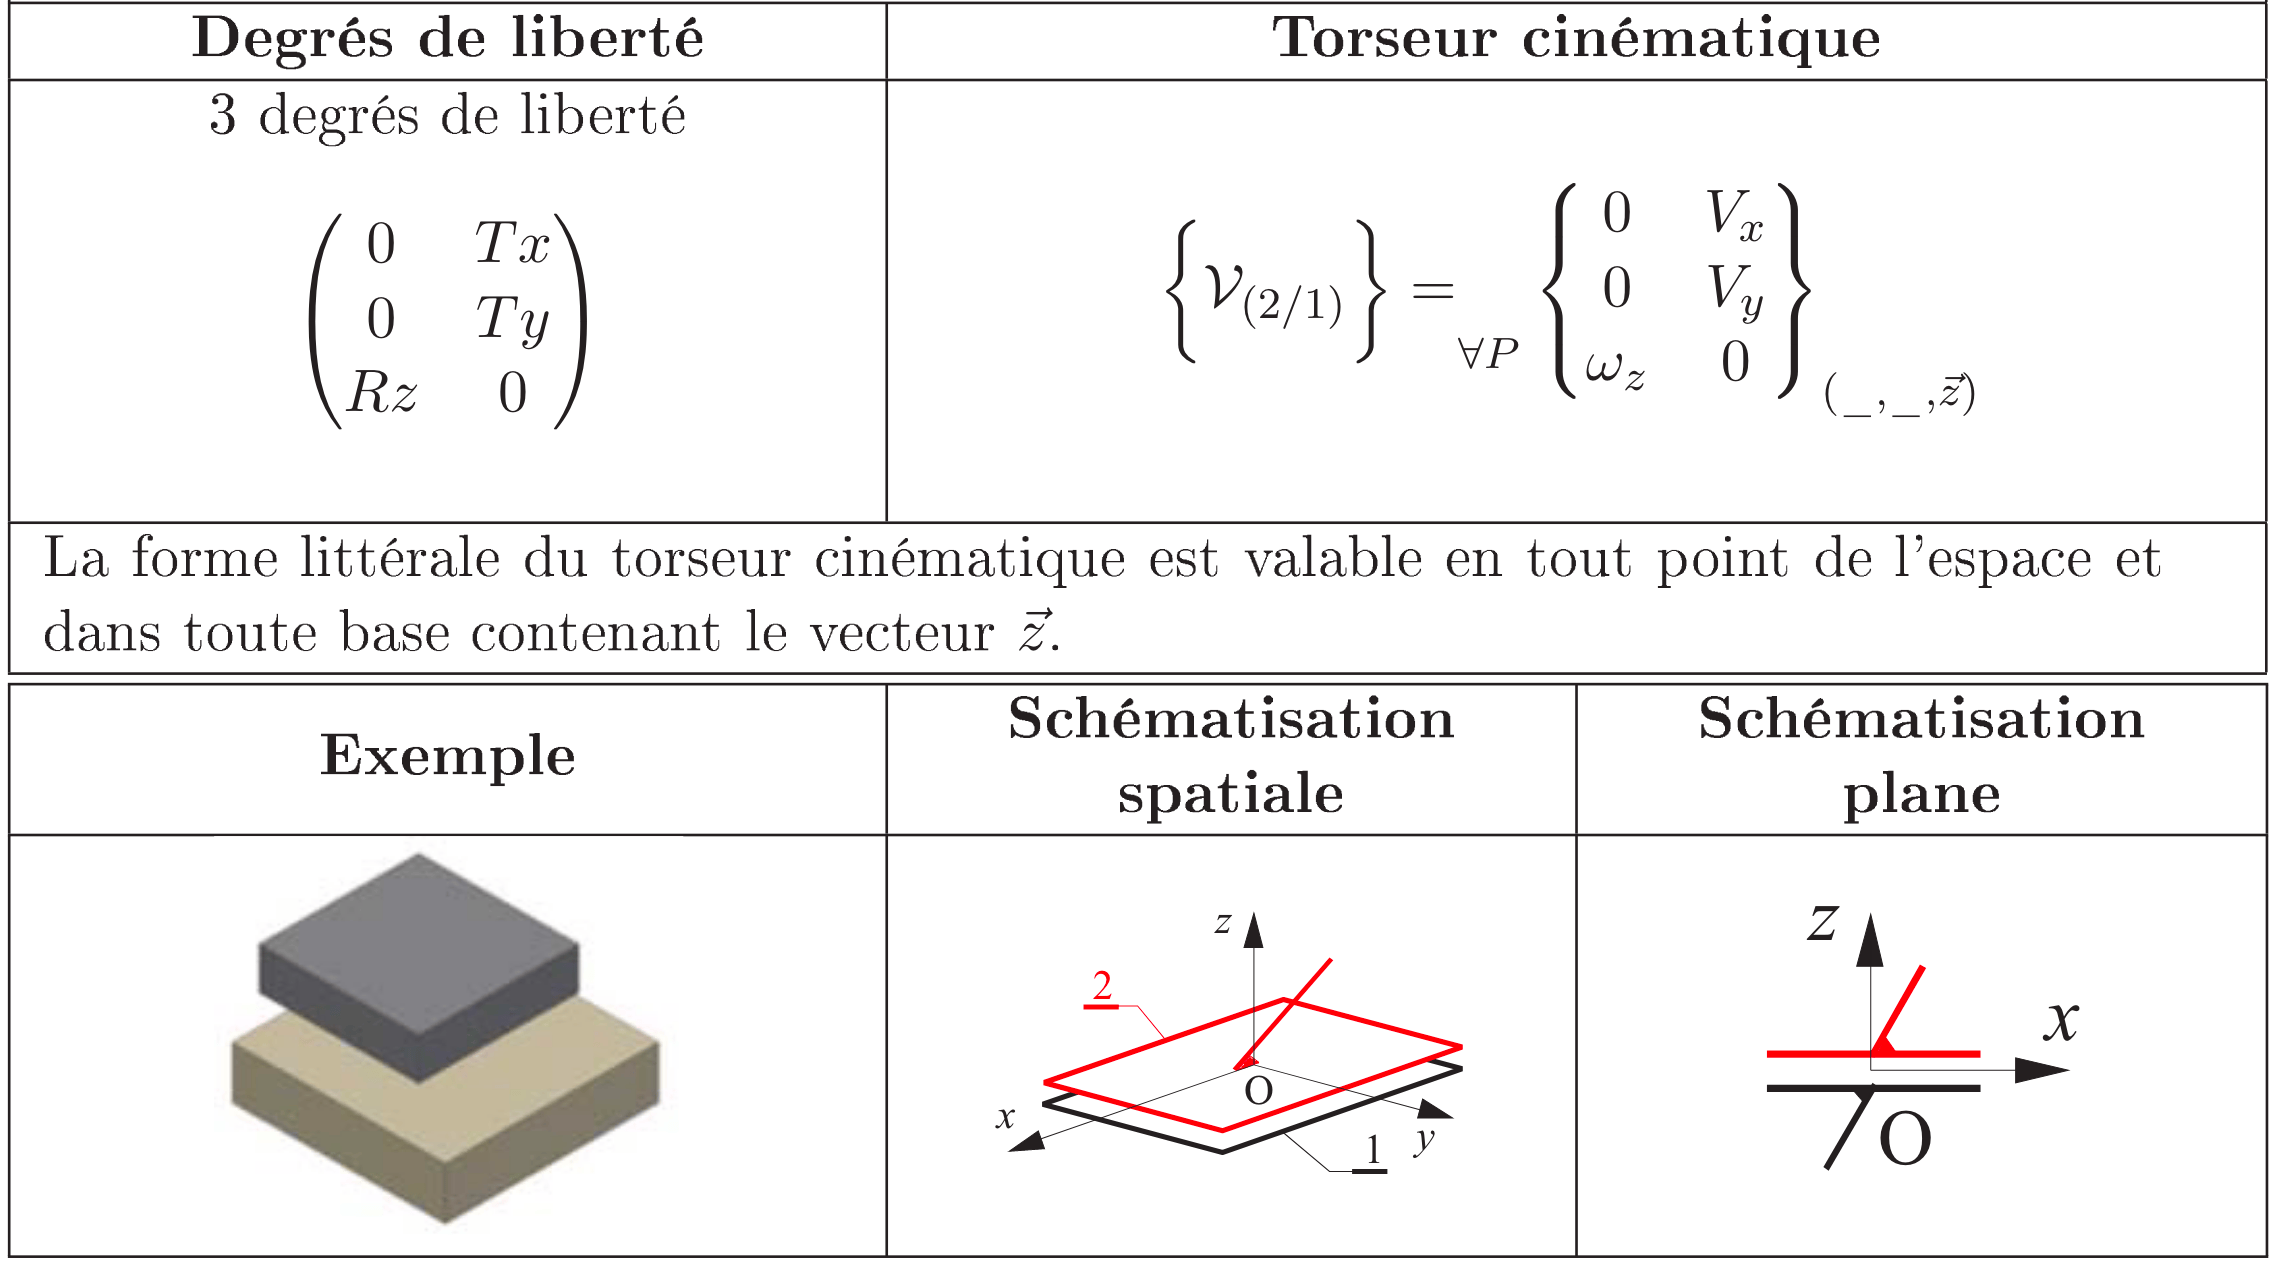
\includegraphics[width=0.7\textwidth,height=\textheight]{CM3/Liaison-Plan-01.png}
\end{center}
\end{block}
\end{frame}

\begin{frame}{Liste de liaisons standard}
\phantomsection\label{liste-de-liaisons-standard}
\begin{center}
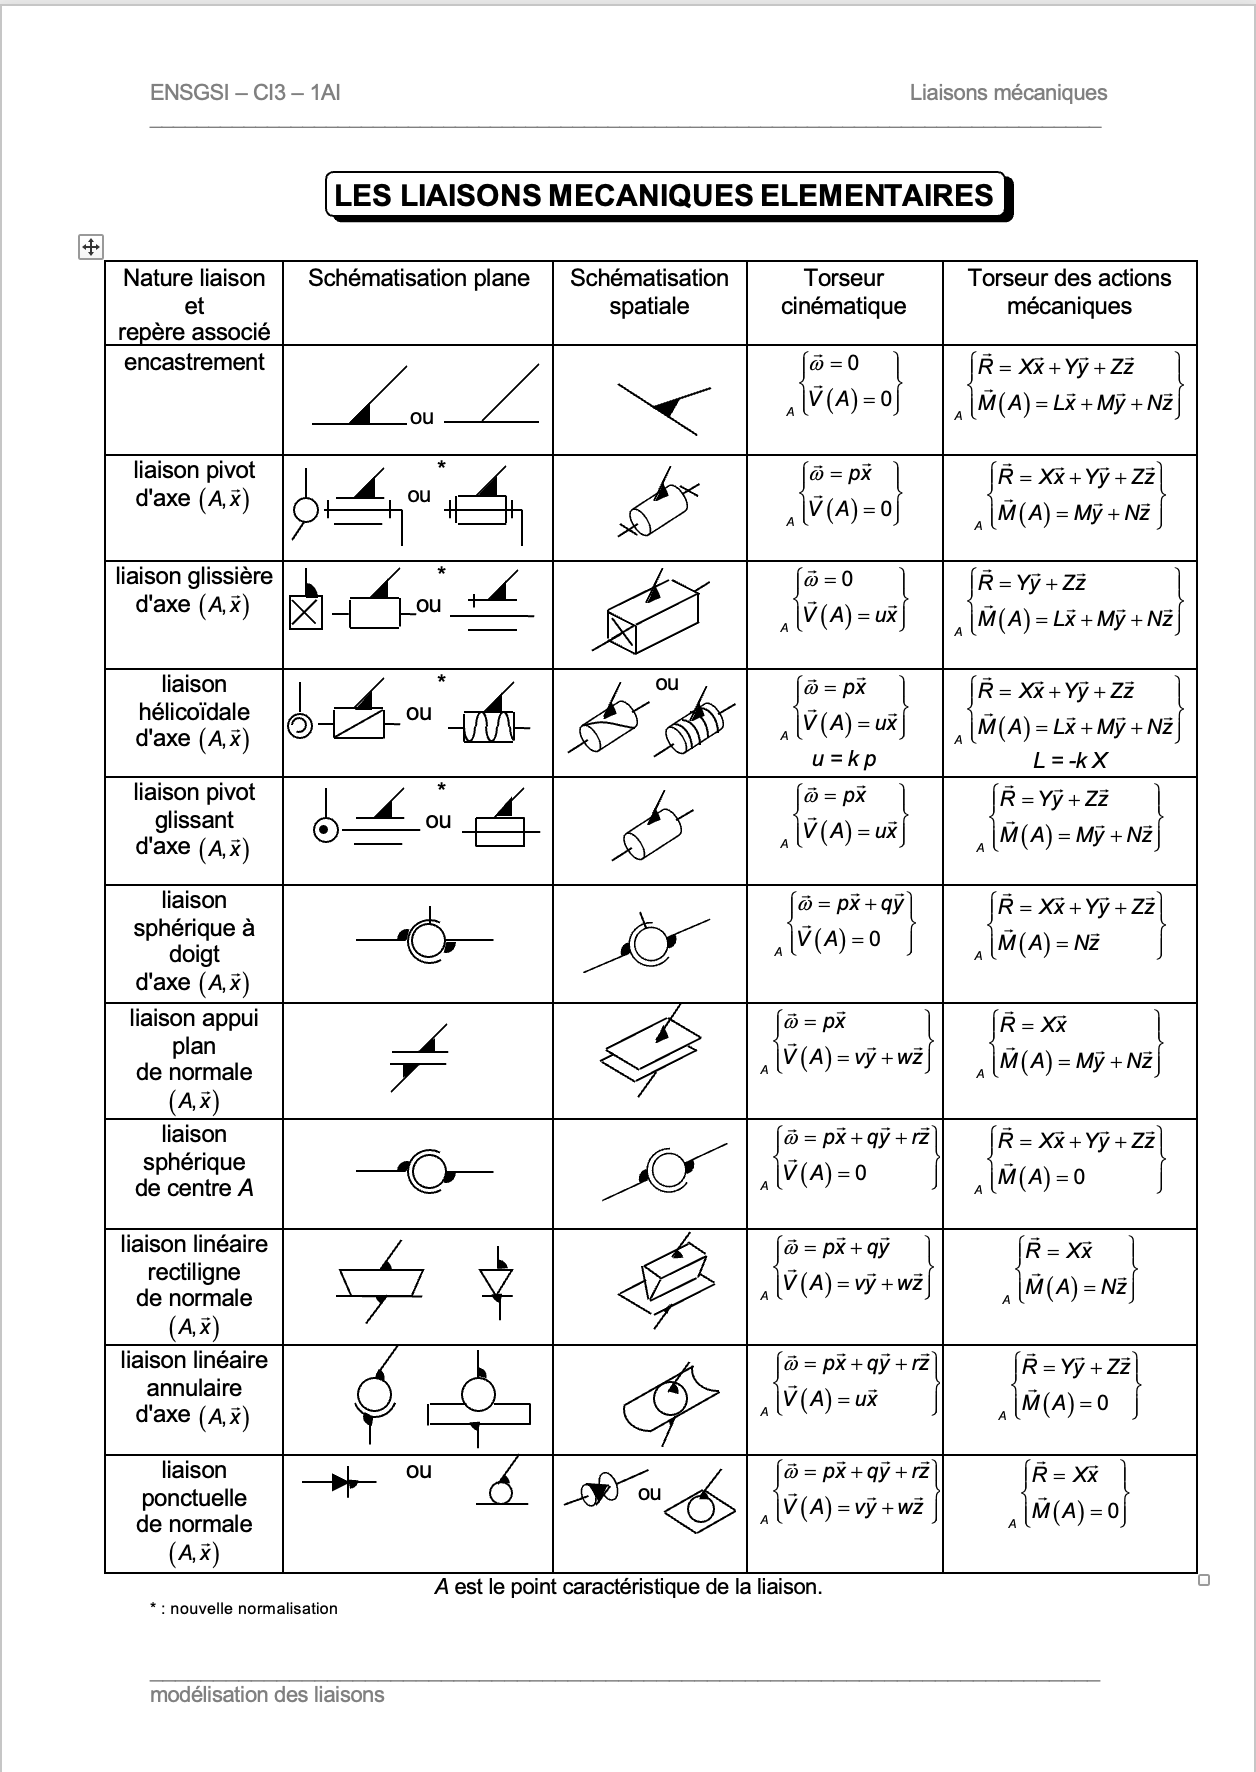
\includegraphics[width=0.7\textwidth,height=\textheight]{CM3/Liaisons.png}
\end{center}
\end{frame}

\subsection{Pour quoi faire?}\label{pour-quoi-faire}

\begin{frame}{Pour quoi faire?}
. . . Construire un schéma cinématique, une représentation simplifiée
d'un mécanisme permettant \textbf{une meilleure compréhension du
fonctionnement}.
\end{frame}

\section{Élaboration d'un schéma
cinématique}\label{uxe9laboration-dun-schuxe9ma-cinuxe9matique}

\subsection{Définition}\label{duxe9finition}

\begin{frame}{Définition}
Le schéma cinématique d'un mécanisme est un modèle filaire du mécanisme
utilisant les symboles normalisés des liaisons.

Ce modèle est utile tant au niveau de la conception que de l'analyse à
posteriori pour réaliser l'étude cinématique ou dynamique (trajectoire,
vitesse, efforts, etc.)
\end{frame}

\subsection{Example 1}\label{example-1}

\begin{frame}{Example 1}
\textbf{Modélisation cinématique d'un micromoteur de modélisme}
\end{frame}

\begin{frame}{Etapes}
\phantomsection\label{etapes}
\begin{enumerate}
\tightlist
\item
  Regroupement des pièces en ensembles solides
\item
  Élaboration du graphe des liaisons
\item
  Construction du schéma cinématique
\end{enumerate}
\end{frame}

\begin{frame}{Etapes}
\phantomsection\label{etapes-1}
\begin{enumerate}
\tightlist
\item
  \textbf{Regroupement des pièces en ensembles solides}
\item
  {Élaboration du graphe des liaisons}
\item
  {Construction du schéma cinématique}
\end{enumerate}

\begin{figure}

\begin{minipage}{0.70\linewidth}
🔎 On regroupe les pièces dans des ensembles (appelés classes
d'équivalence cinématique)✍️ Un nom (un numéro par exemple)🔵 Une
couleur\end{minipage}%

\end{figure}%
\end{frame}

\begin{frame}{Etapes}
\phantomsection\label{etapes-2}
\begin{enumerate}
\tightlist
\item
  {Regroupement des pièces en ensembles solides}
\item
  \textbf{Élaboration du graphe des liaisons}
\item
  {Construction du schéma cinématique}
\end{enumerate}

\begin{figure}

\begin{minipage}{0.70\linewidth}
✓ Choix d'une base pour le solide de référence (bâti) ✓ Recherche des
contacts entre les solides ✓ Étude des liaisons entre les
solides\end{minipage}%
%
\begin{minipage}{0.30\linewidth}
\begin{center}
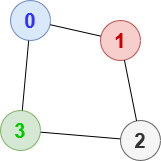
\includegraphics[width=0.5\textwidth,height=\textheight]{CM3/Graphe-des-liaisons.png}
\end{center}
\end{minipage}%

\end{figure}%
\end{frame}

\begin{frame}{Etapes}
\phantomsection\label{etapes-3}
\begin{enumerate}
\tightlist
\item
  {Regroupement des pièces en ensembles solides}
\item
  \textbf{Élaboration du graphe des liaisons}
\item
  {Construction du schéma cinématique}
\end{enumerate}

\begin{figure}

\begin{minipage}{0.80\linewidth}
Analyser pour \textbf{\emph{chaque laiaison}}✓ Surfaces en contact →
(plan/plan, sphère/cylindre, \ldots) ✓ Degrés de liberté ✓
Identification de composants\end{minipage}%

\end{figure}%
\end{frame}

\begin{frame}{Etapes}
\phantomsection\label{etapes-4}
\begin{enumerate}
\tightlist
\item
  {Regroupement des pièces en ensembles solides}
\item
  \textbf{Élaboration du graphe des liaisons}
\item
  {Construction du schéma cinématique}
\end{enumerate}

\begin{figure}

\begin{minipage}{0.80\linewidth}
Analyser pour \textbf{\emph{chaque laiaison}}\(L_{0-1}\) : Pivot d'axe
\((𝐴,\vec{z})\) \(L_{1-2}\) : Pivot d'axe \((𝐵,\vec{z})\) \(L_{2-3}\) :
Pivot glissant d'axe \((𝐶,\vec{z})\) \(L_{3-0}\) : Pivot glissant d'axe
\((𝐴,\vec{y})\)\end{minipage}%

\end{figure}%
\end{frame}

\begin{frame}{Etapes}
\phantomsection\label{etapes-5}
\begin{enumerate}
\tightlist
\item
  {Regroupement des pièces en ensembles solides}
\item
  {Élaboration du graphe des liaisons}
\item
  \textbf{Construction du schéma cinématique}
\end{enumerate}

\begin{figure}

\begin{minipage}{0.80\linewidth}
✓ Tracé des éléments de situation des liaisons {✓ Dessin des symboles
des liaisons} {✓ Simuler}\end{minipage}%

\end{figure}%
\end{frame}

\begin{frame}{Etapes}
\phantomsection\label{etapes-6}
\begin{enumerate}
\tightlist
\item
  {Regroupement des pièces en ensembles solides}
\item
  {Élaboration du graphe des liaisons}
\item
  \textbf{Construction du schéma cinématique}
\end{enumerate}

\begin{figure}

\begin{minipage}{0.80\linewidth}
{✓ Tracé des éléments de situation des liaisons} ✓ Dessin des symboles
des liaisons {✓ Simuler}\end{minipage}%

\end{figure}%
\end{frame}

\begin{frame}{Etapes}
\phantomsection\label{etapes-7}
\begin{enumerate}
\tightlist
\item
  {Regroupement des pièces en ensembles solides}
\item
  {Élaboration du graphe des liaisons}
\item
  \textbf{Construction du schéma cinématique}
\end{enumerate}

\begin{figure}

\begin{minipage}{0.80\linewidth}
{✓ Tracé des éléments de situation des liaisons} {✓ Dessin des symboles
des liaisons} ✓ Simuler\end{minipage}%

\end{figure}%
\end{frame}

\subsection{💻 Simuler pour mieux
comprendre.}\label{simuler-pour-mieux-comprendre.}

\begin{frame}{💻 Simuler pour mieux comprendre.}
\begin{figure}

\begin{minipage}{0.56\linewidth}
Introduction to Mechanism Design Source:
\url{http://www.mechdes.net/}\end{minipage}%
%
\begin{minipage}{0.44\linewidth}
\begin{center}
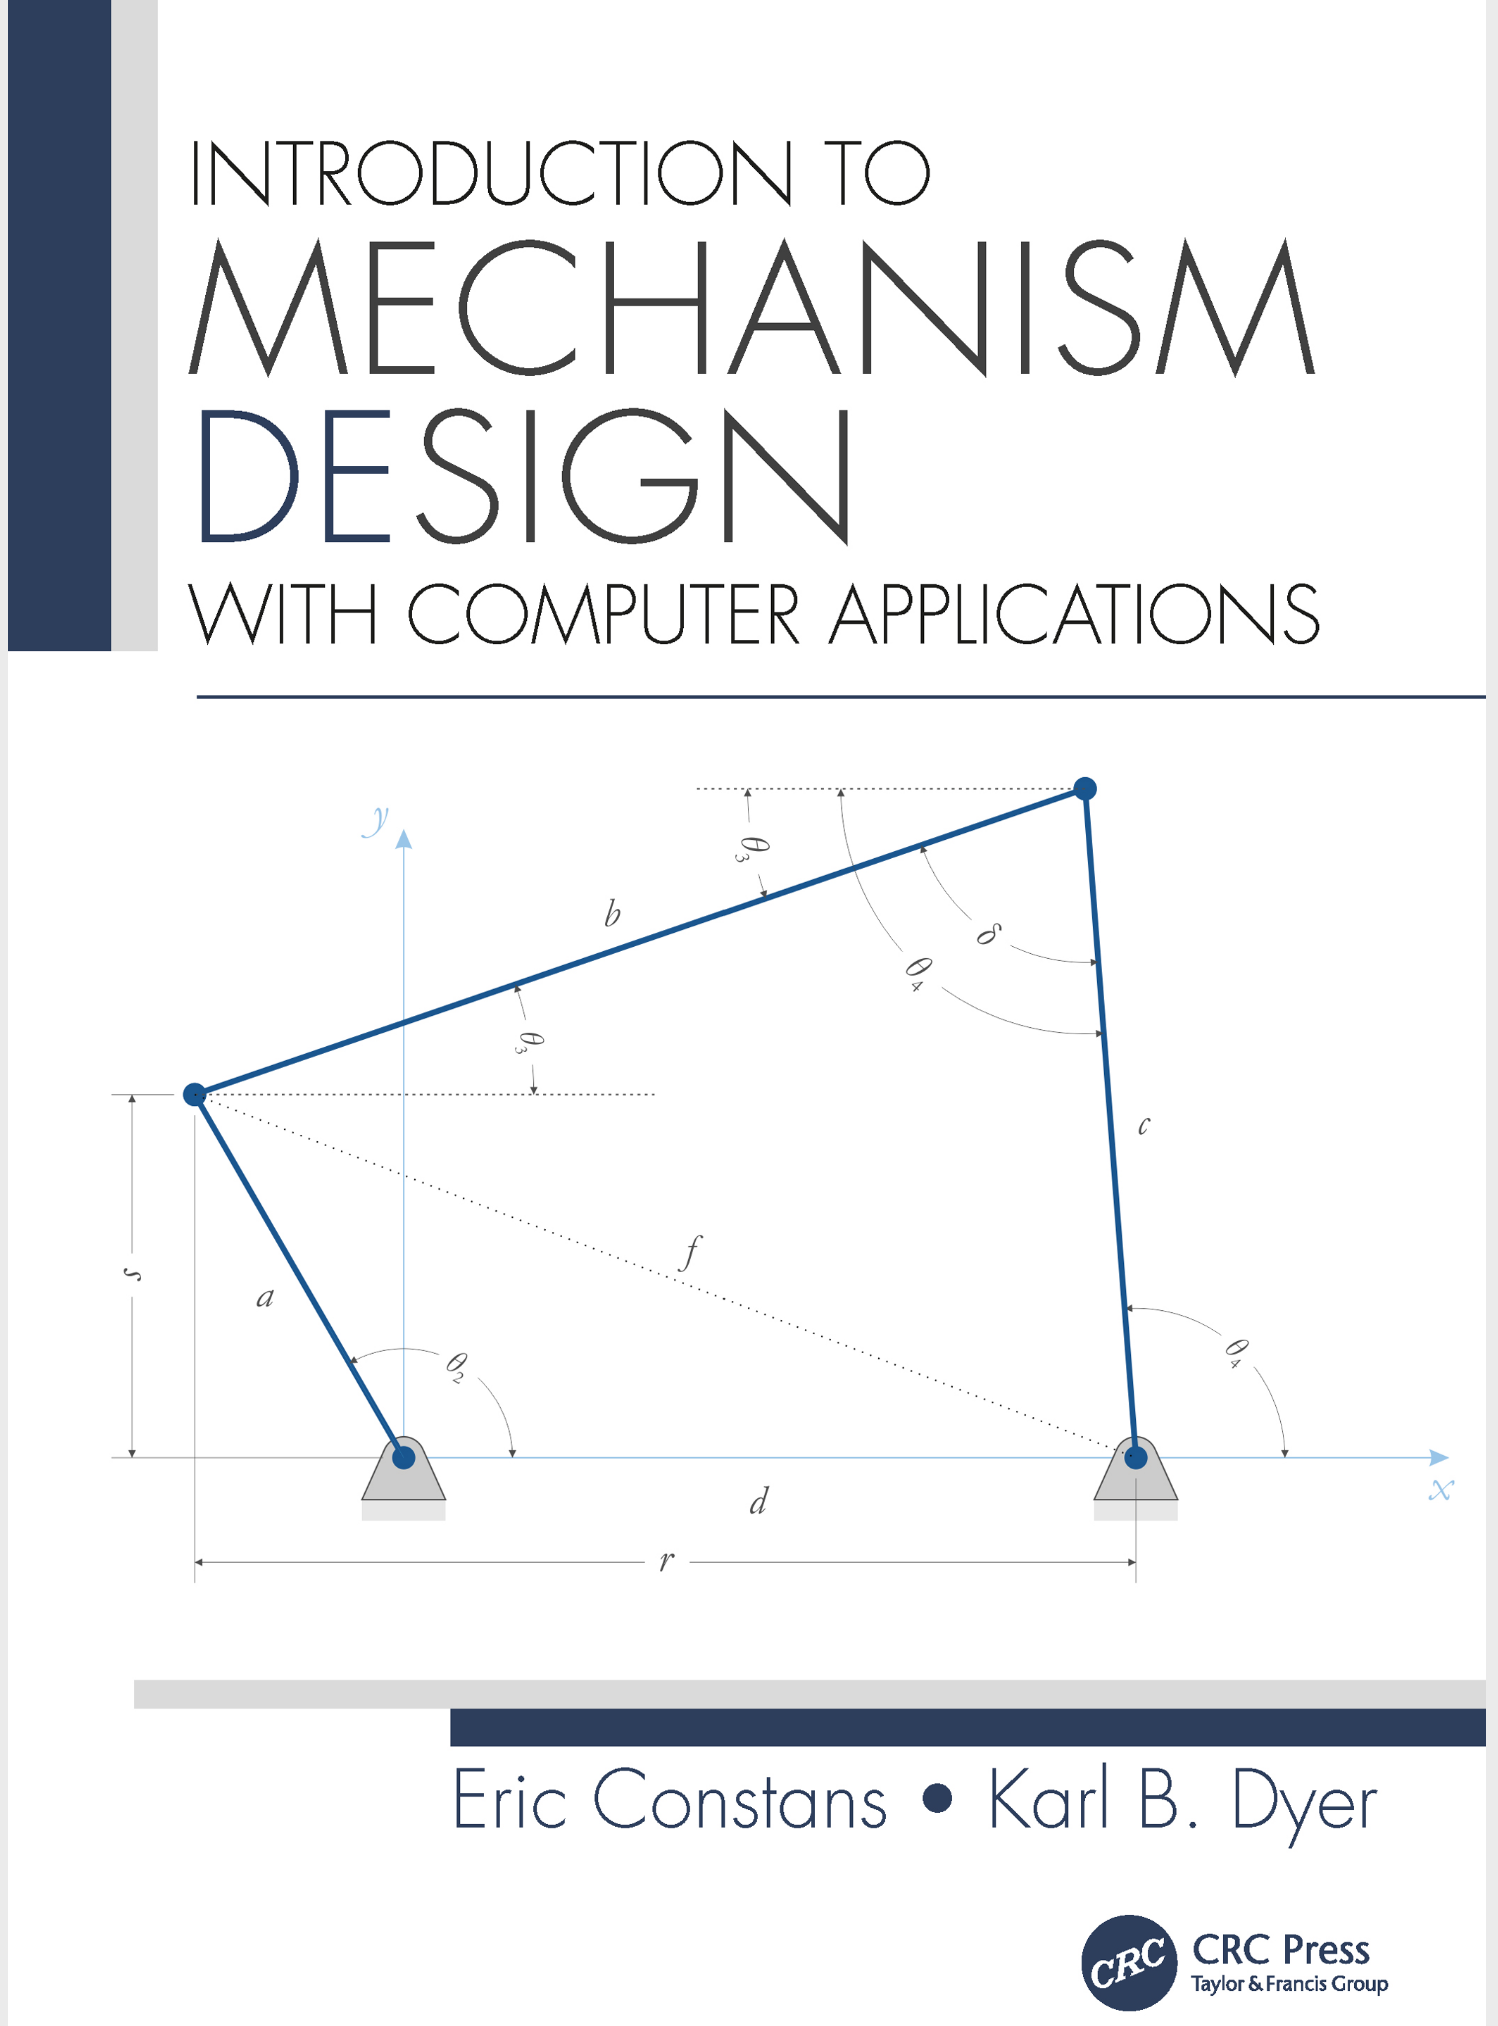
\includegraphics[width=0.8\textwidth,height=\textheight]{CM3/Mechanism-design.png}
\end{center}
\end{minipage}%

\end{figure}%
\end{frame}

\subsection{Example 2: Vélo elliptique
VE680}\label{example-2-vuxe9lo-elliptique-ve680}

\subsection{Example 2: Vélo elliptique
VE680}\label{example-2-vuxe9lo-elliptique-ve680-1}

\begin{frame}{Example 2: Vélo elliptique VE680}
\begin{block}{Contexte}
\begin{figure}

\begin{minipage}{0.80\linewidth}
Société Décathlon commercialise le système du vélo elliptique de marque
Domyos, modèle VE 680.\begin{center}
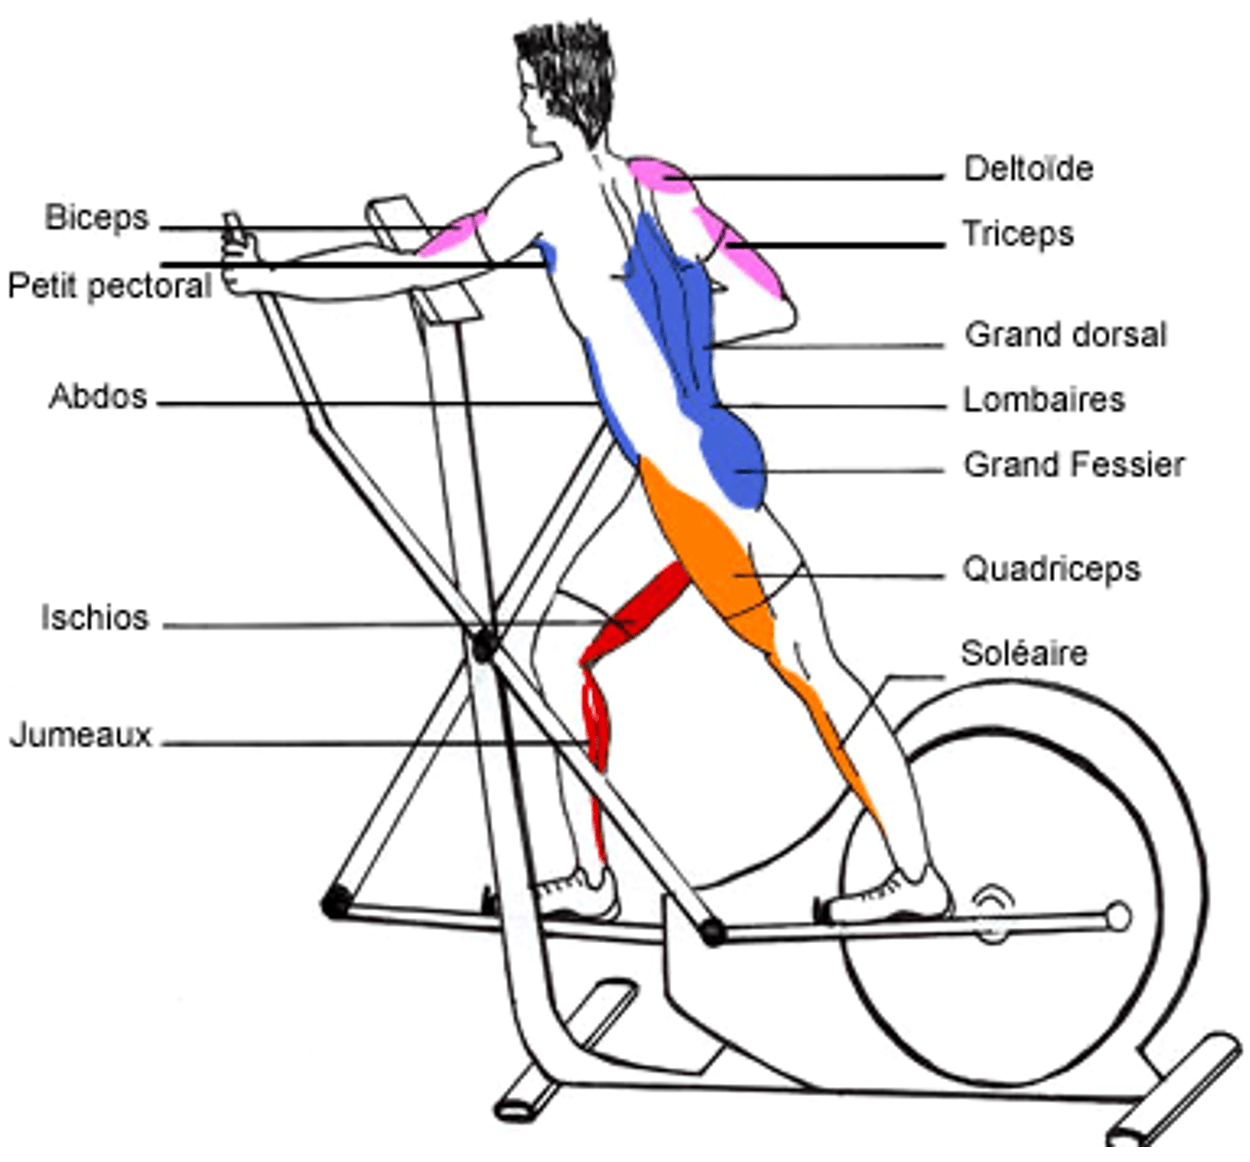
\includegraphics[width=0.4\textwidth,height=\textheight]{CM3/Velo-fonctionnelle.png}
\end{center}
\end{minipage}%
%
\begin{minipage}{0.20\linewidth}
\begin{center}
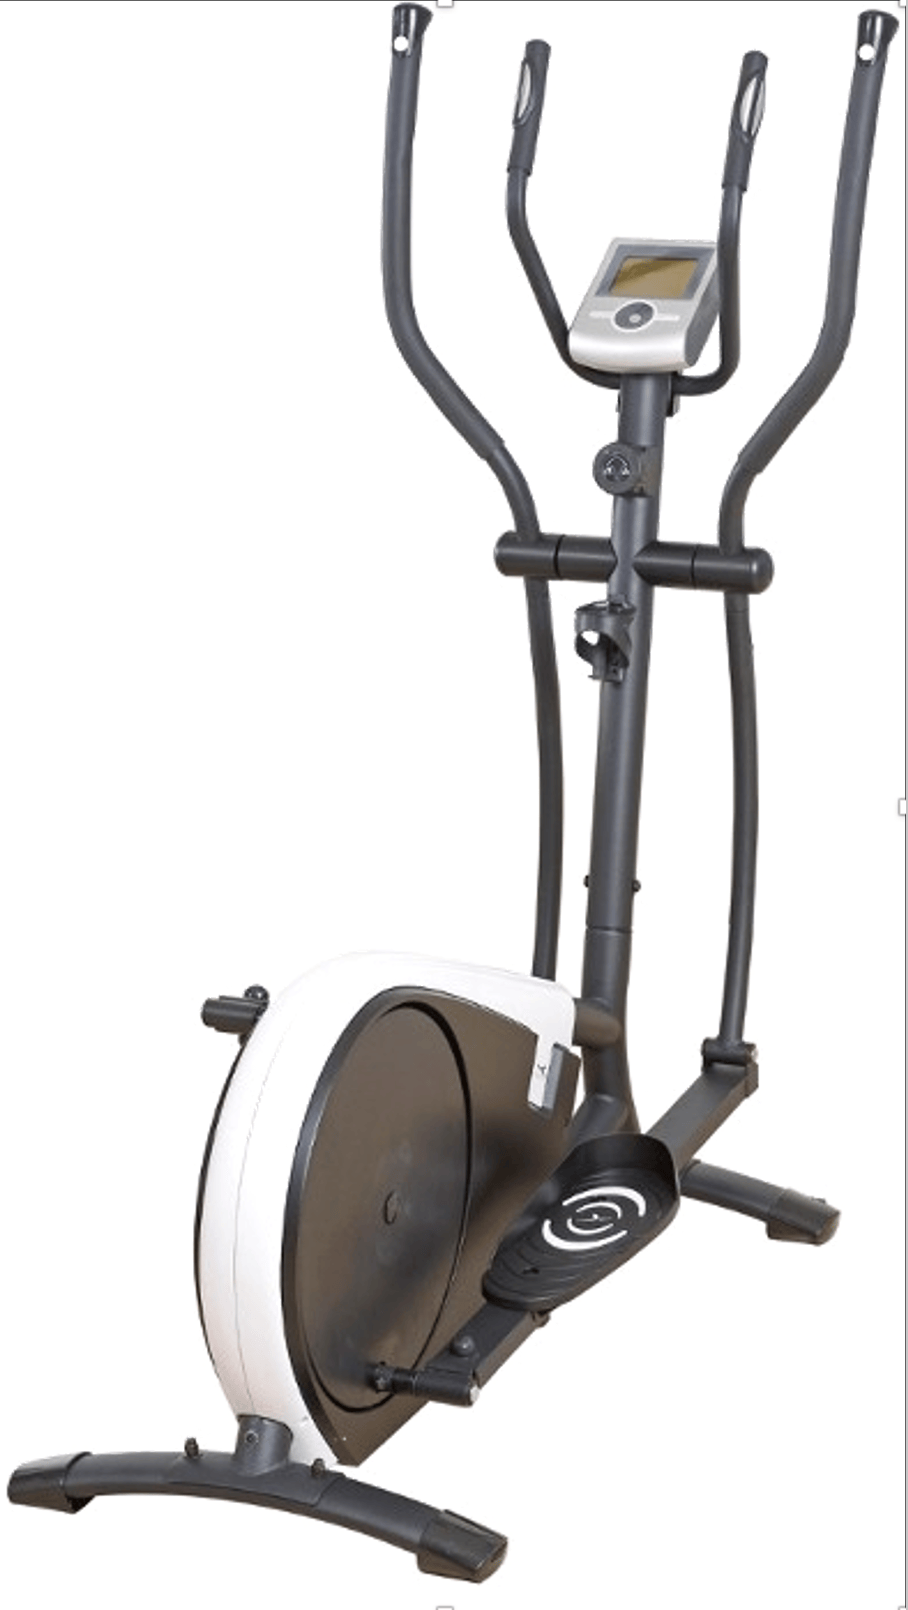
\includegraphics[width=0.7\textwidth,height=\textheight]{CM3/Velo.png}
\end{center}
\end{minipage}%

\end{figure}%
\end{block}

\begin{block}{Analyse du besoin}
\begin{figure}

\begin{minipage}{0.50\linewidth}
\begin{center}
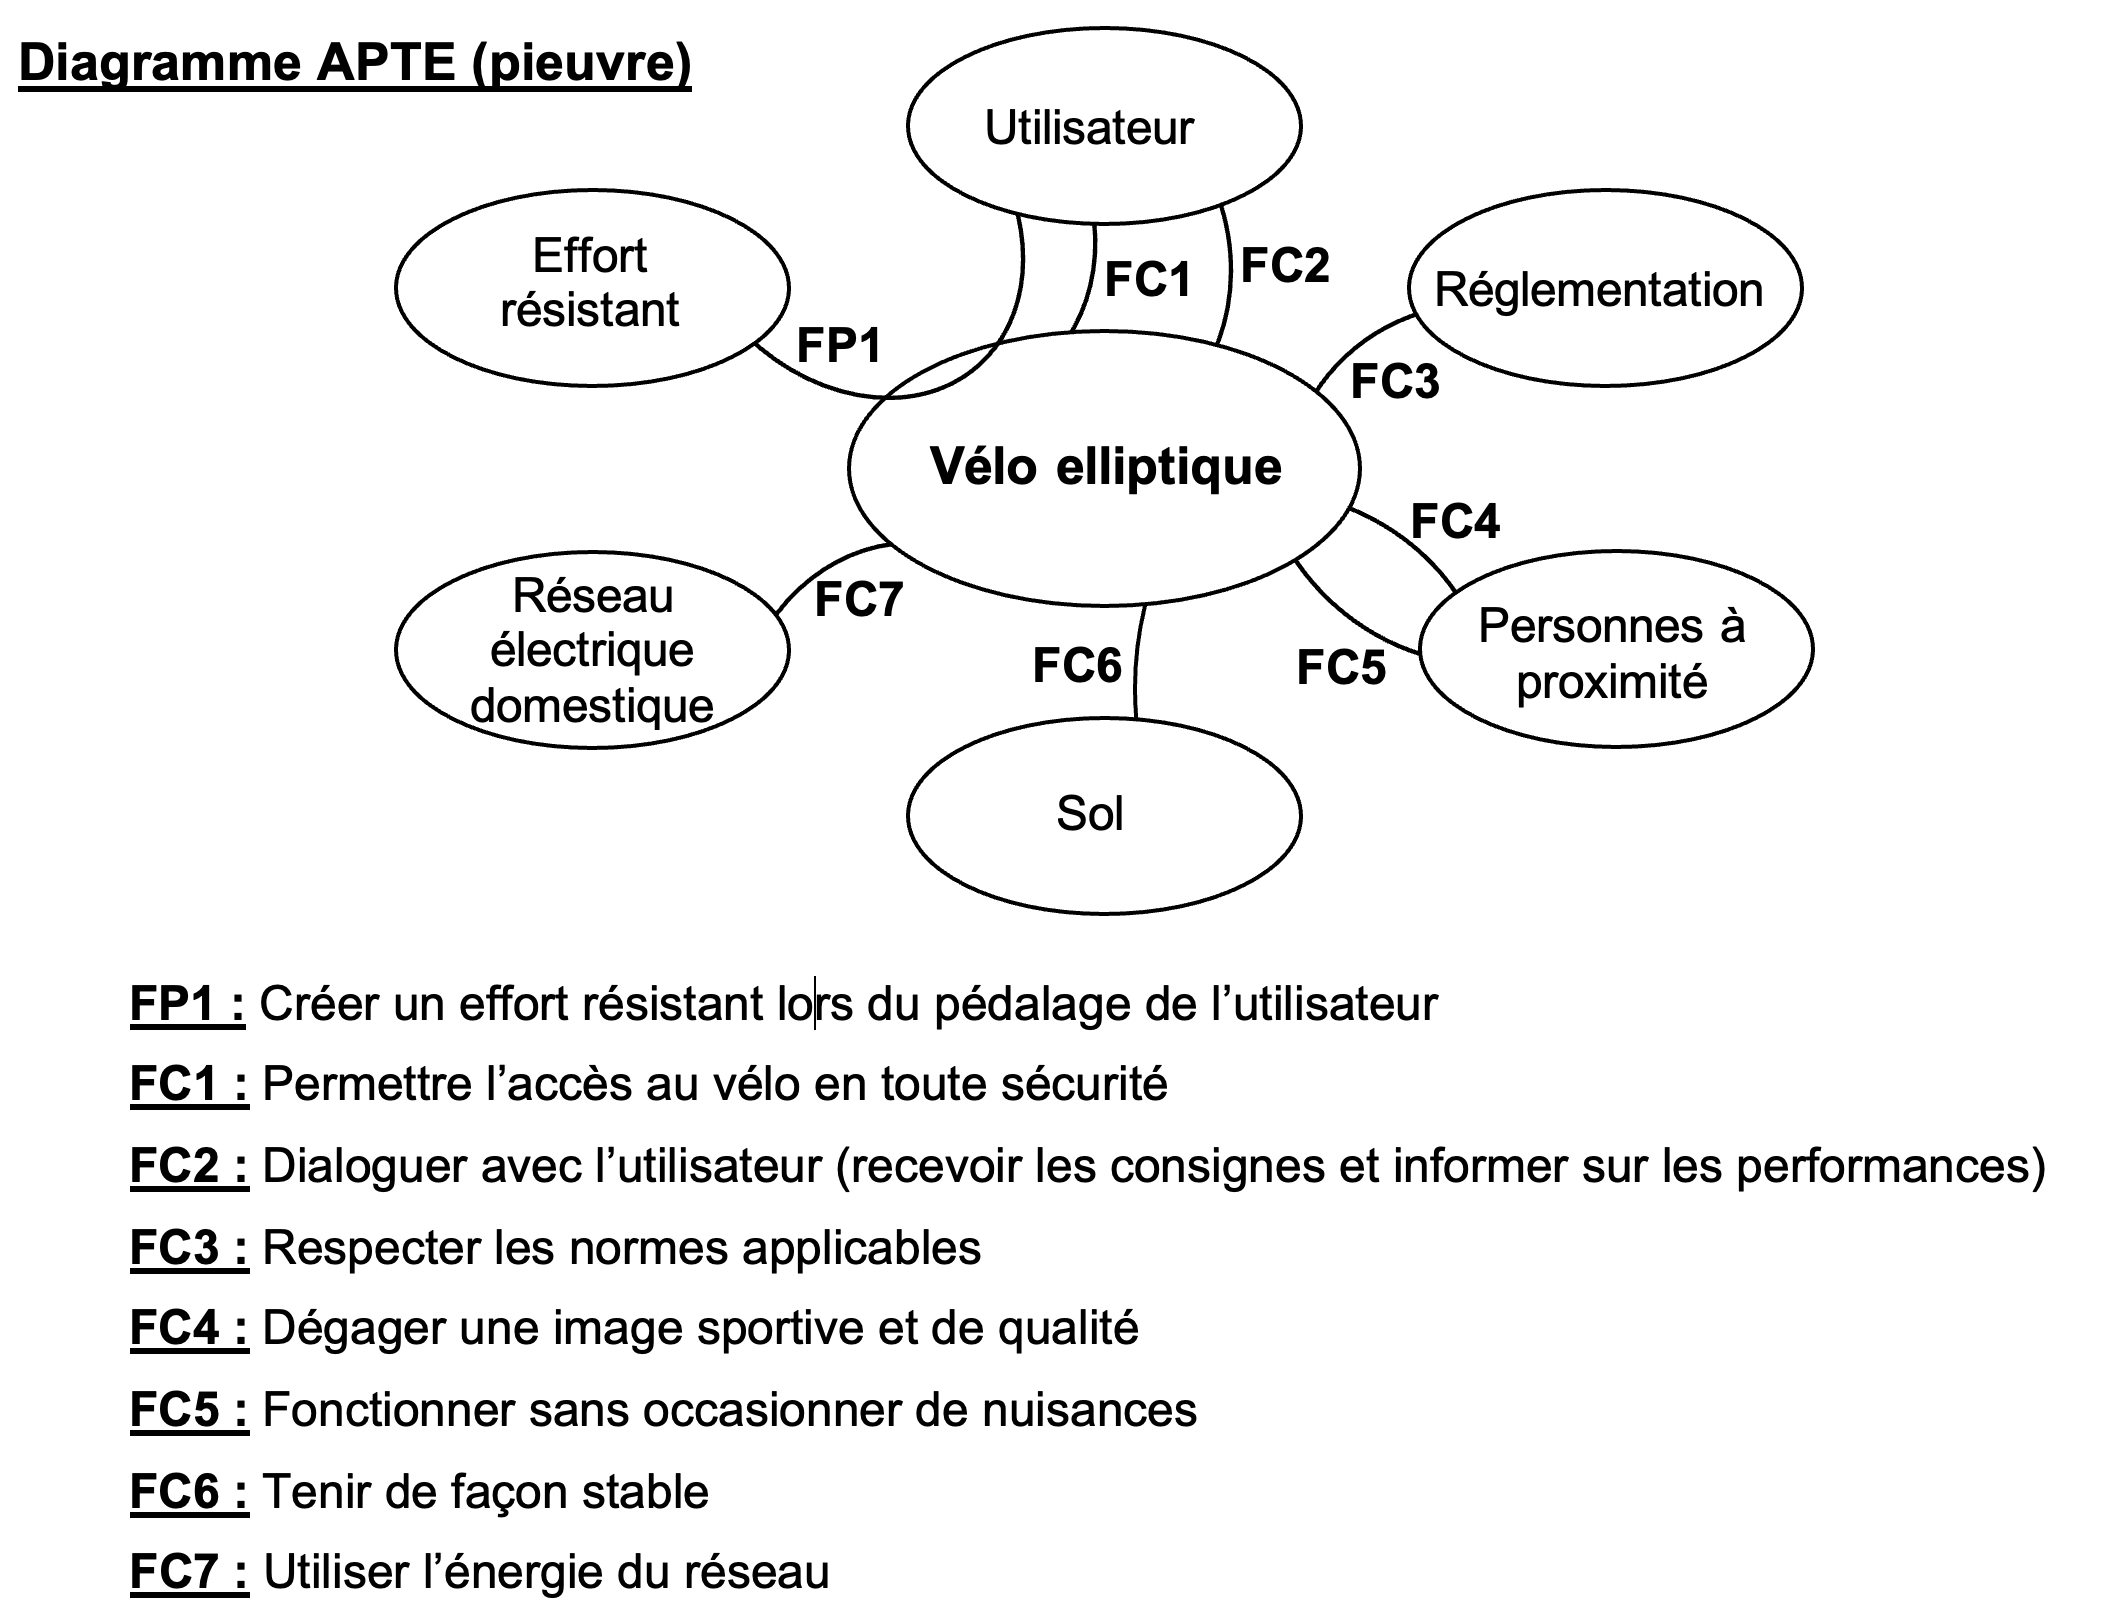
\includegraphics[width=1\textwidth,height=\textheight]{CM3/Velo-fonctionnelle-01.png}
\end{center}
\end{minipage}%
%
\begin{minipage}{0.50\linewidth}
\begin{center}
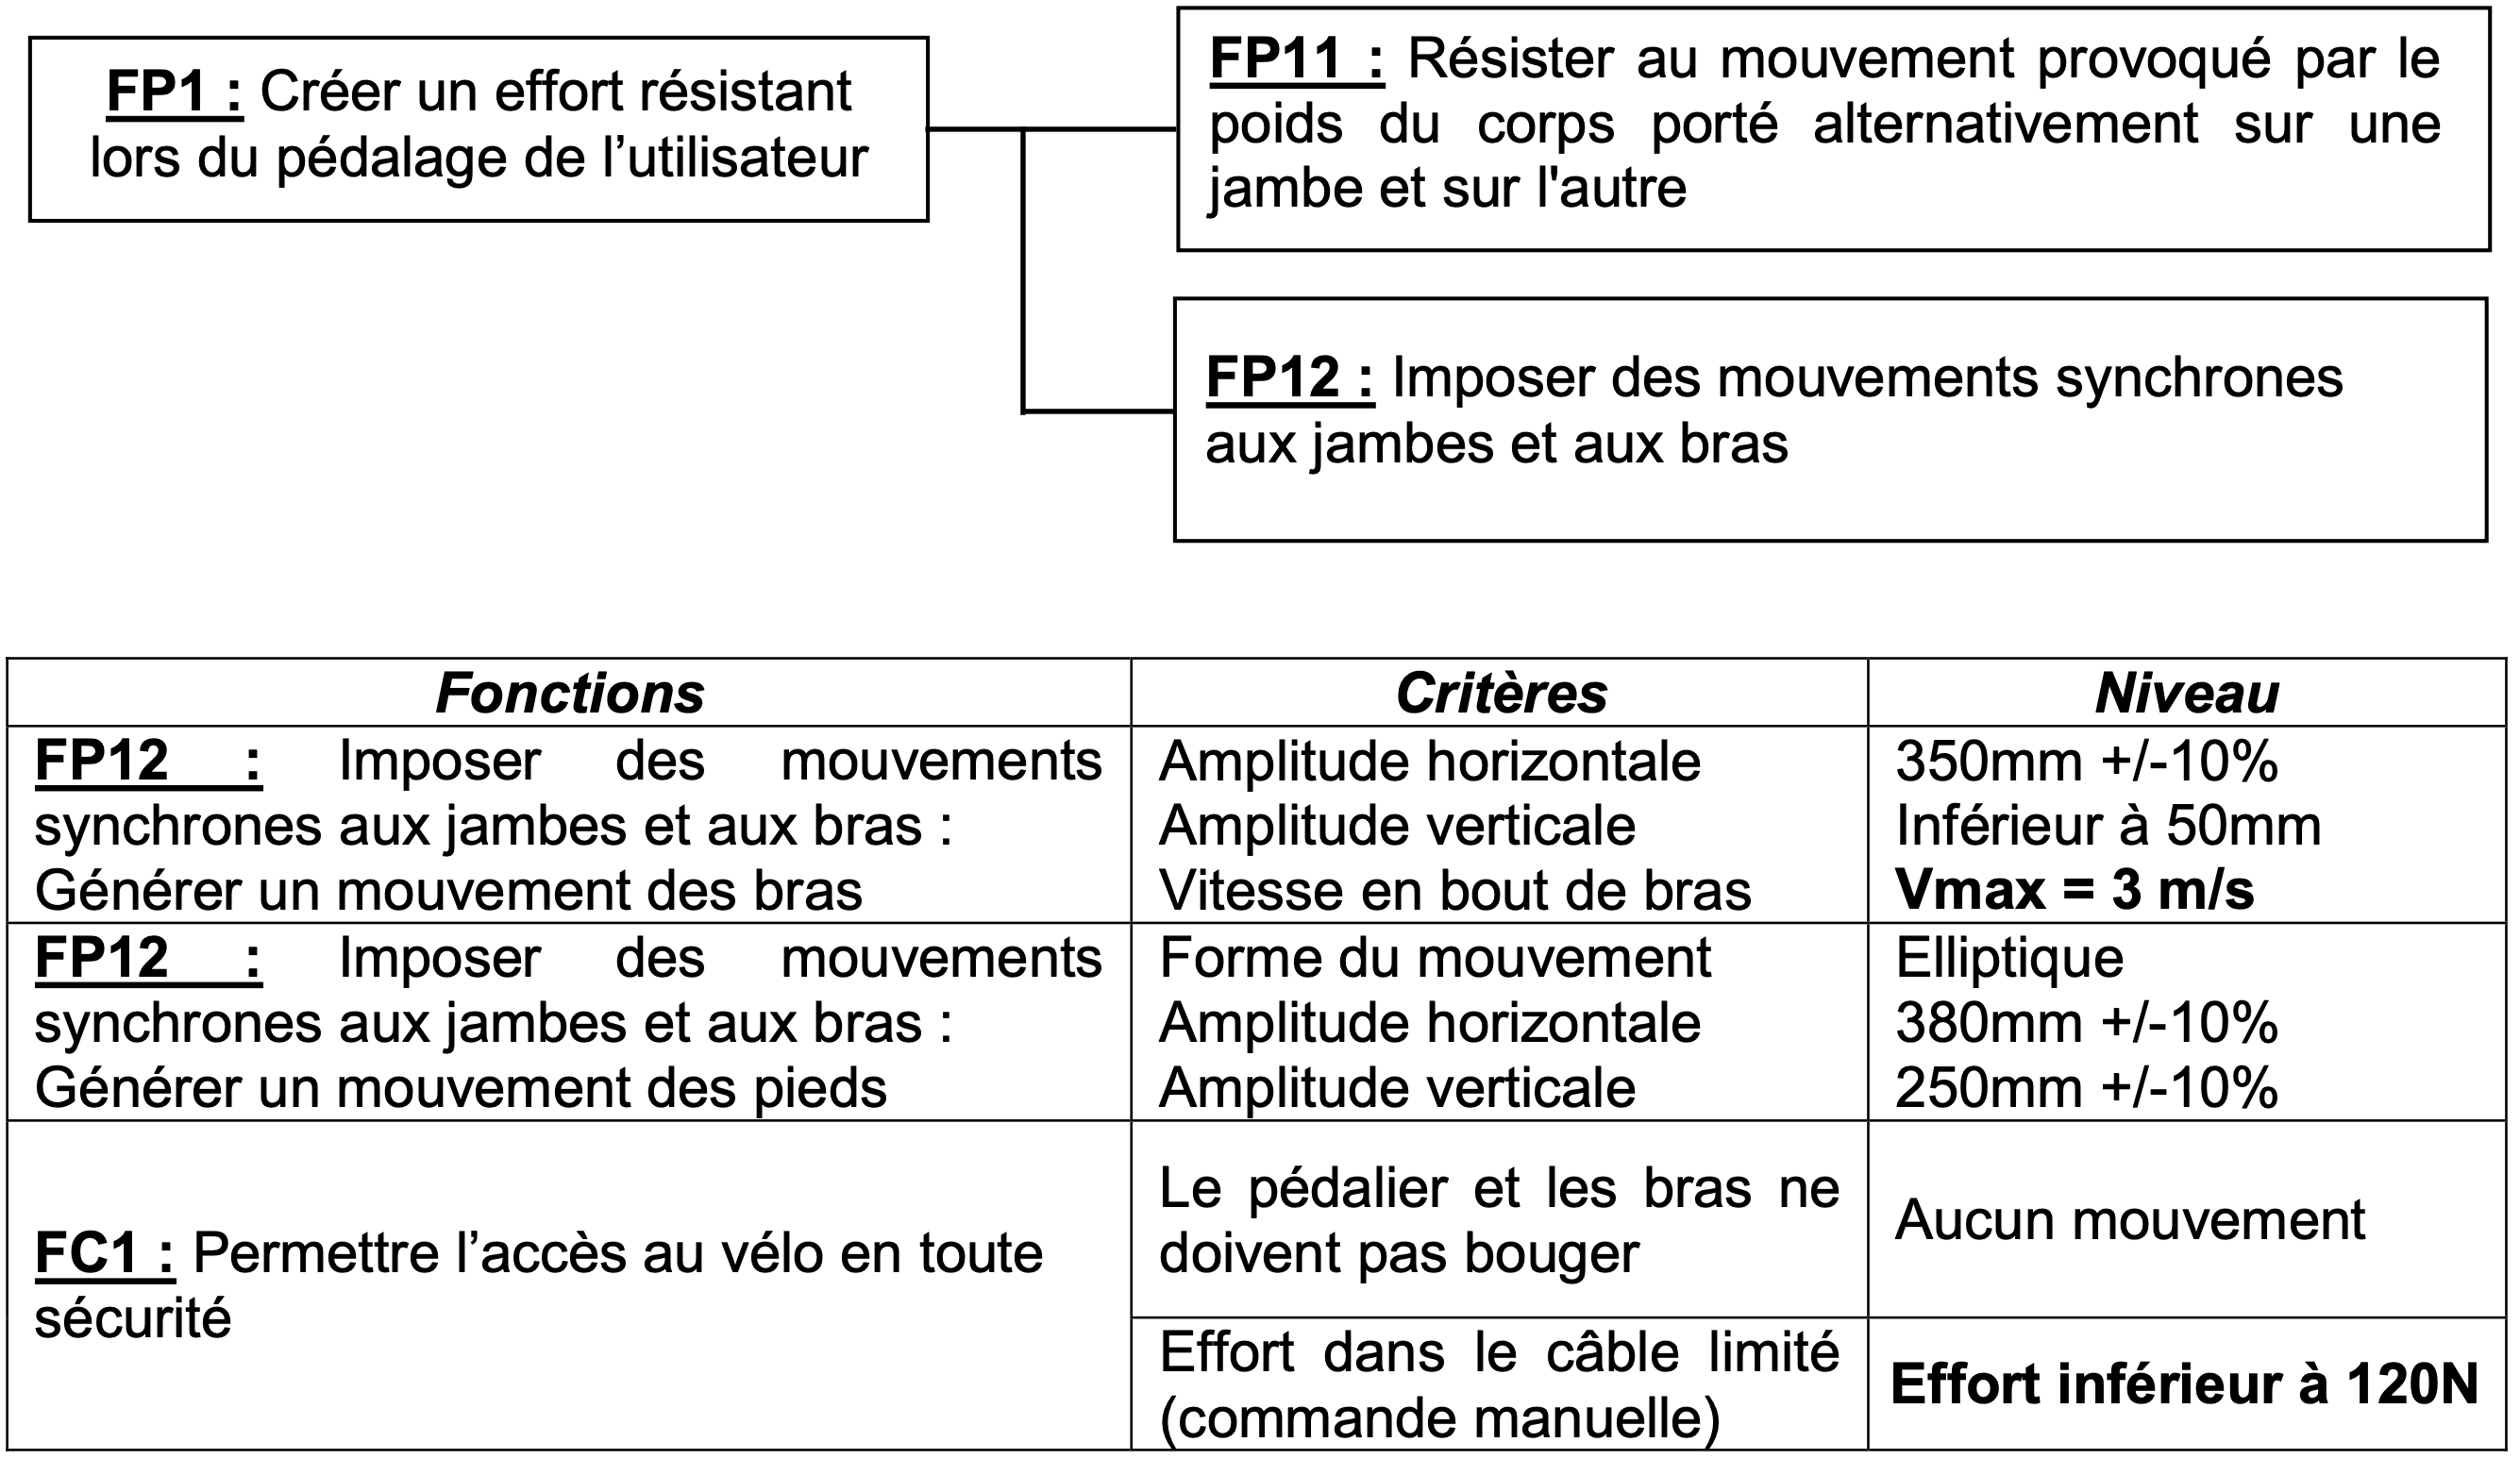
\includegraphics[width=1\textwidth,height=\textheight]{CM3/Velo-fonctionnelle-03.png}
\end{center}
\end{minipage}%

\end{figure}%
\end{block}

\begin{block}{Chaîne d'Energie}
\begin{figure}

\begin{minipage}{0.55\linewidth}
\begin{center}
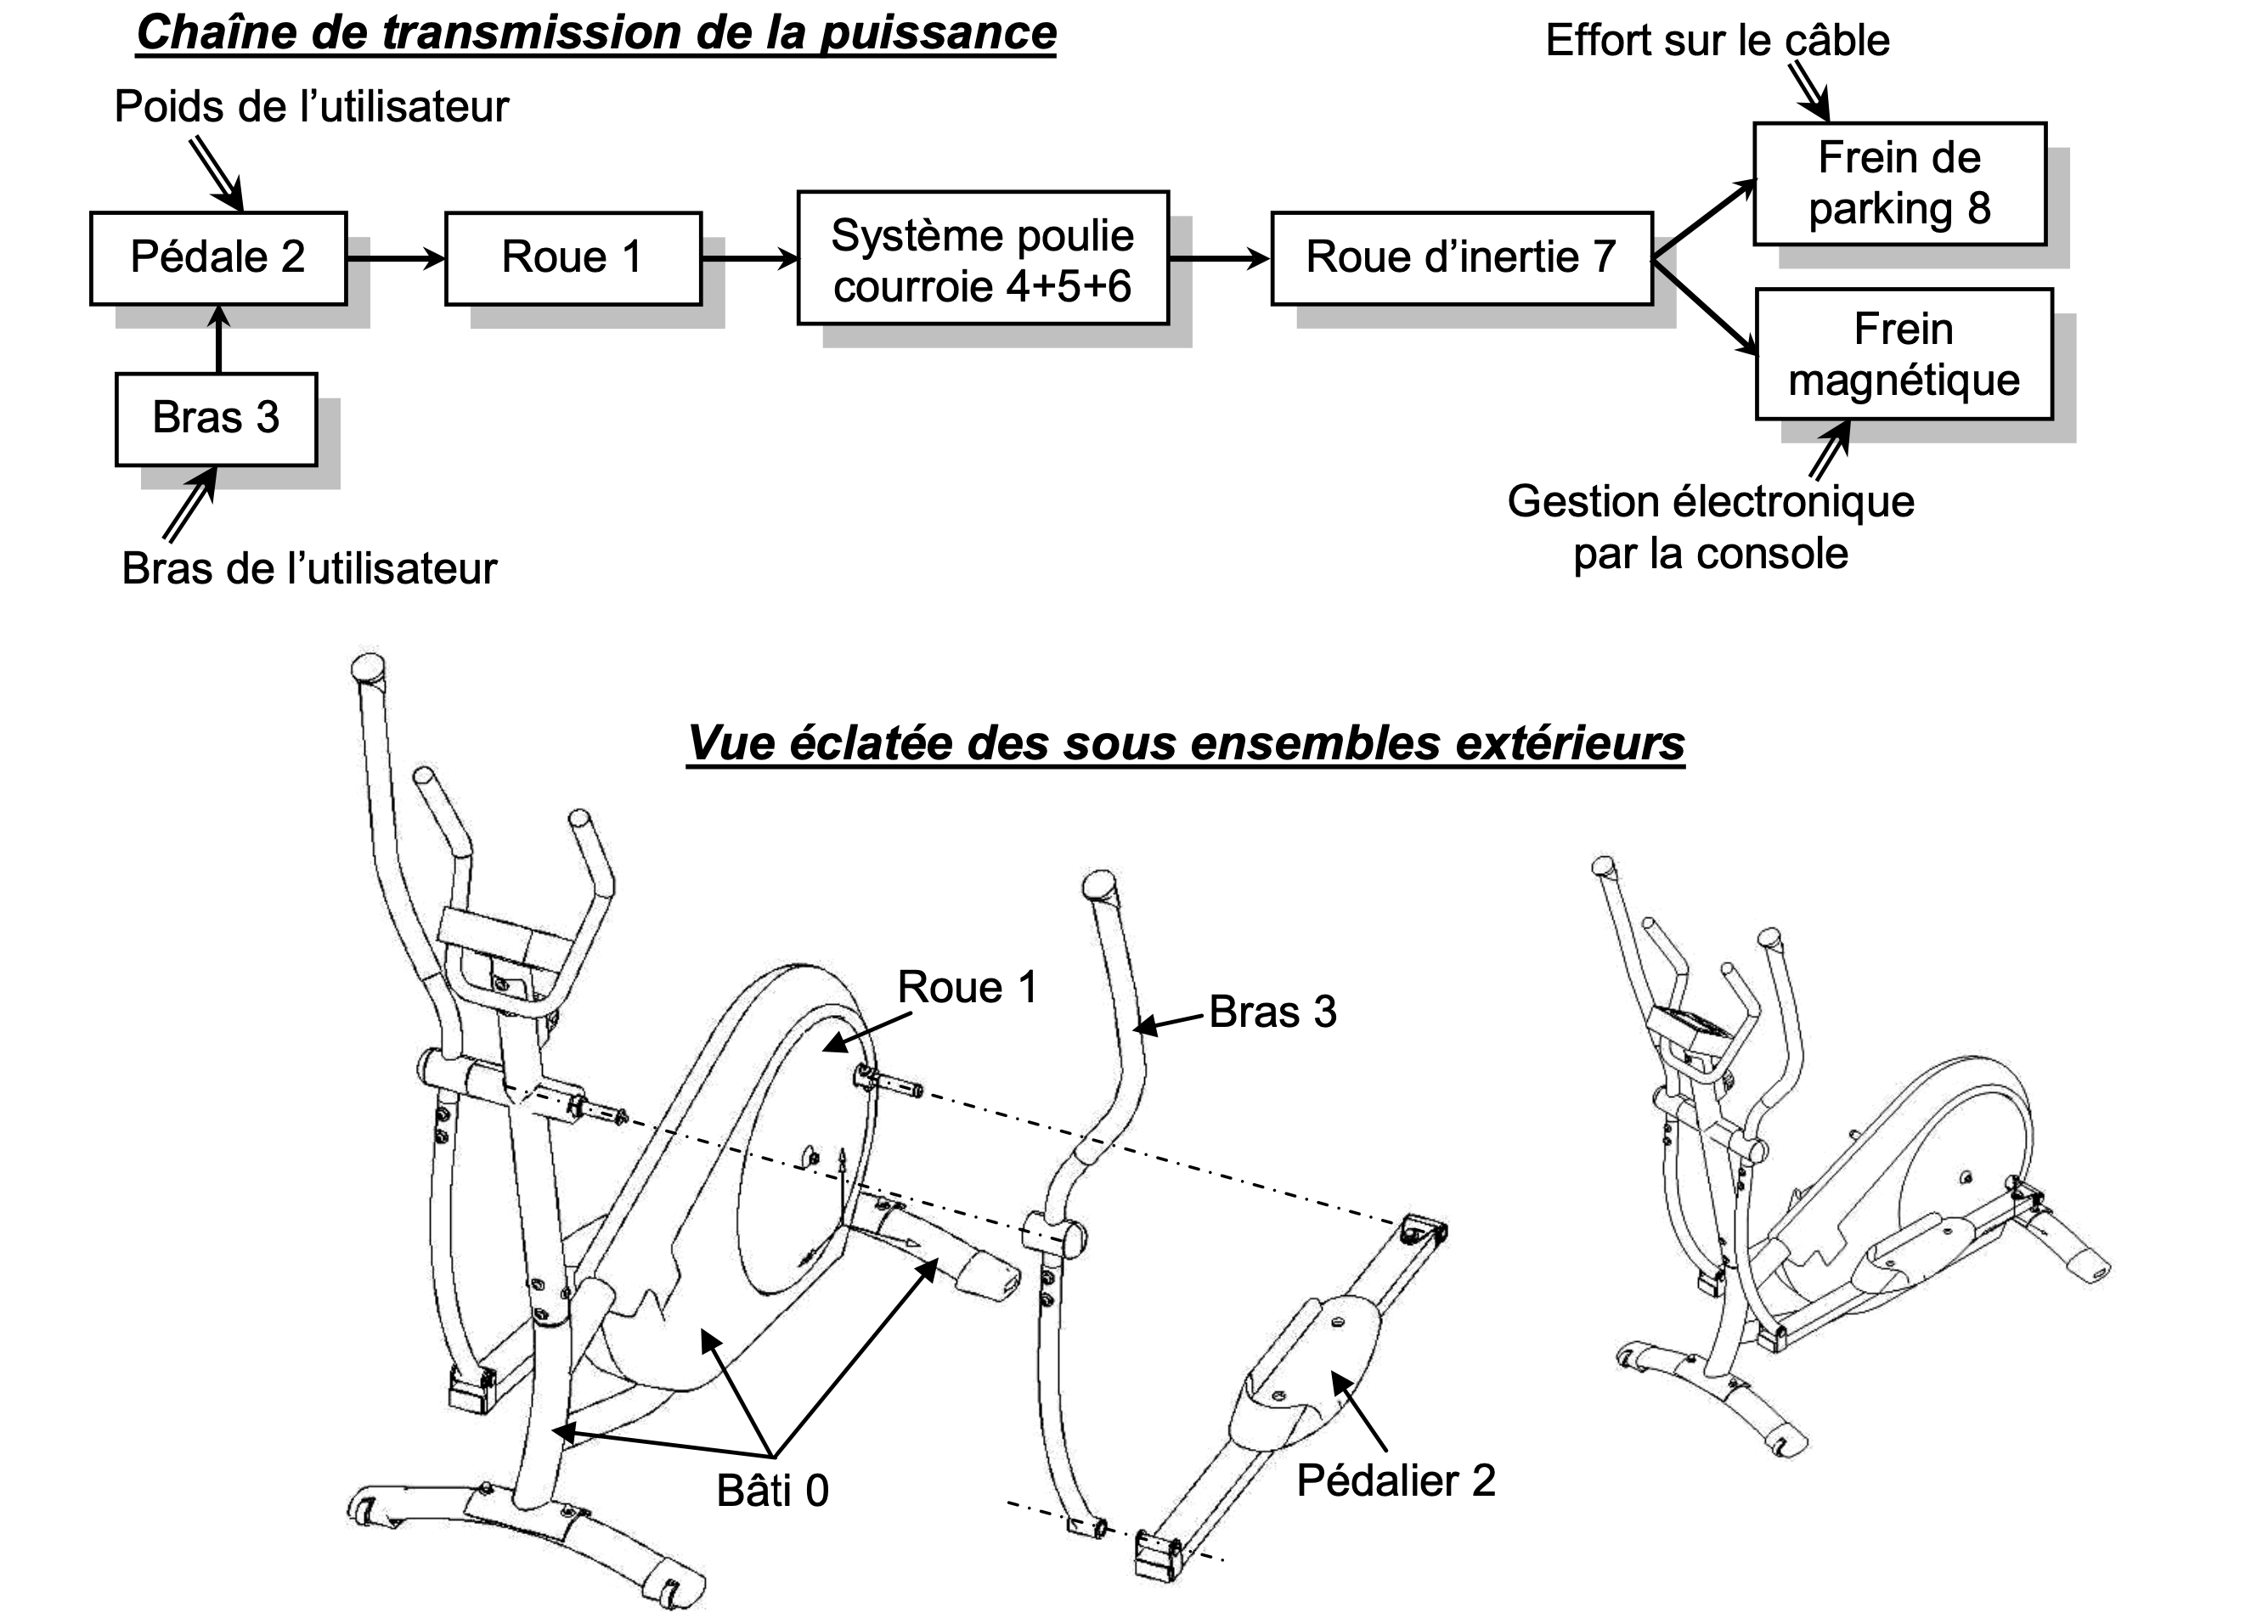
\includegraphics[width=1\textwidth,height=\textheight]{CM3/Velo-fonctionnelle-04.png}
\end{center}
\end{minipage}%
%
\begin{minipage}{0.46\linewidth}
\begin{center}
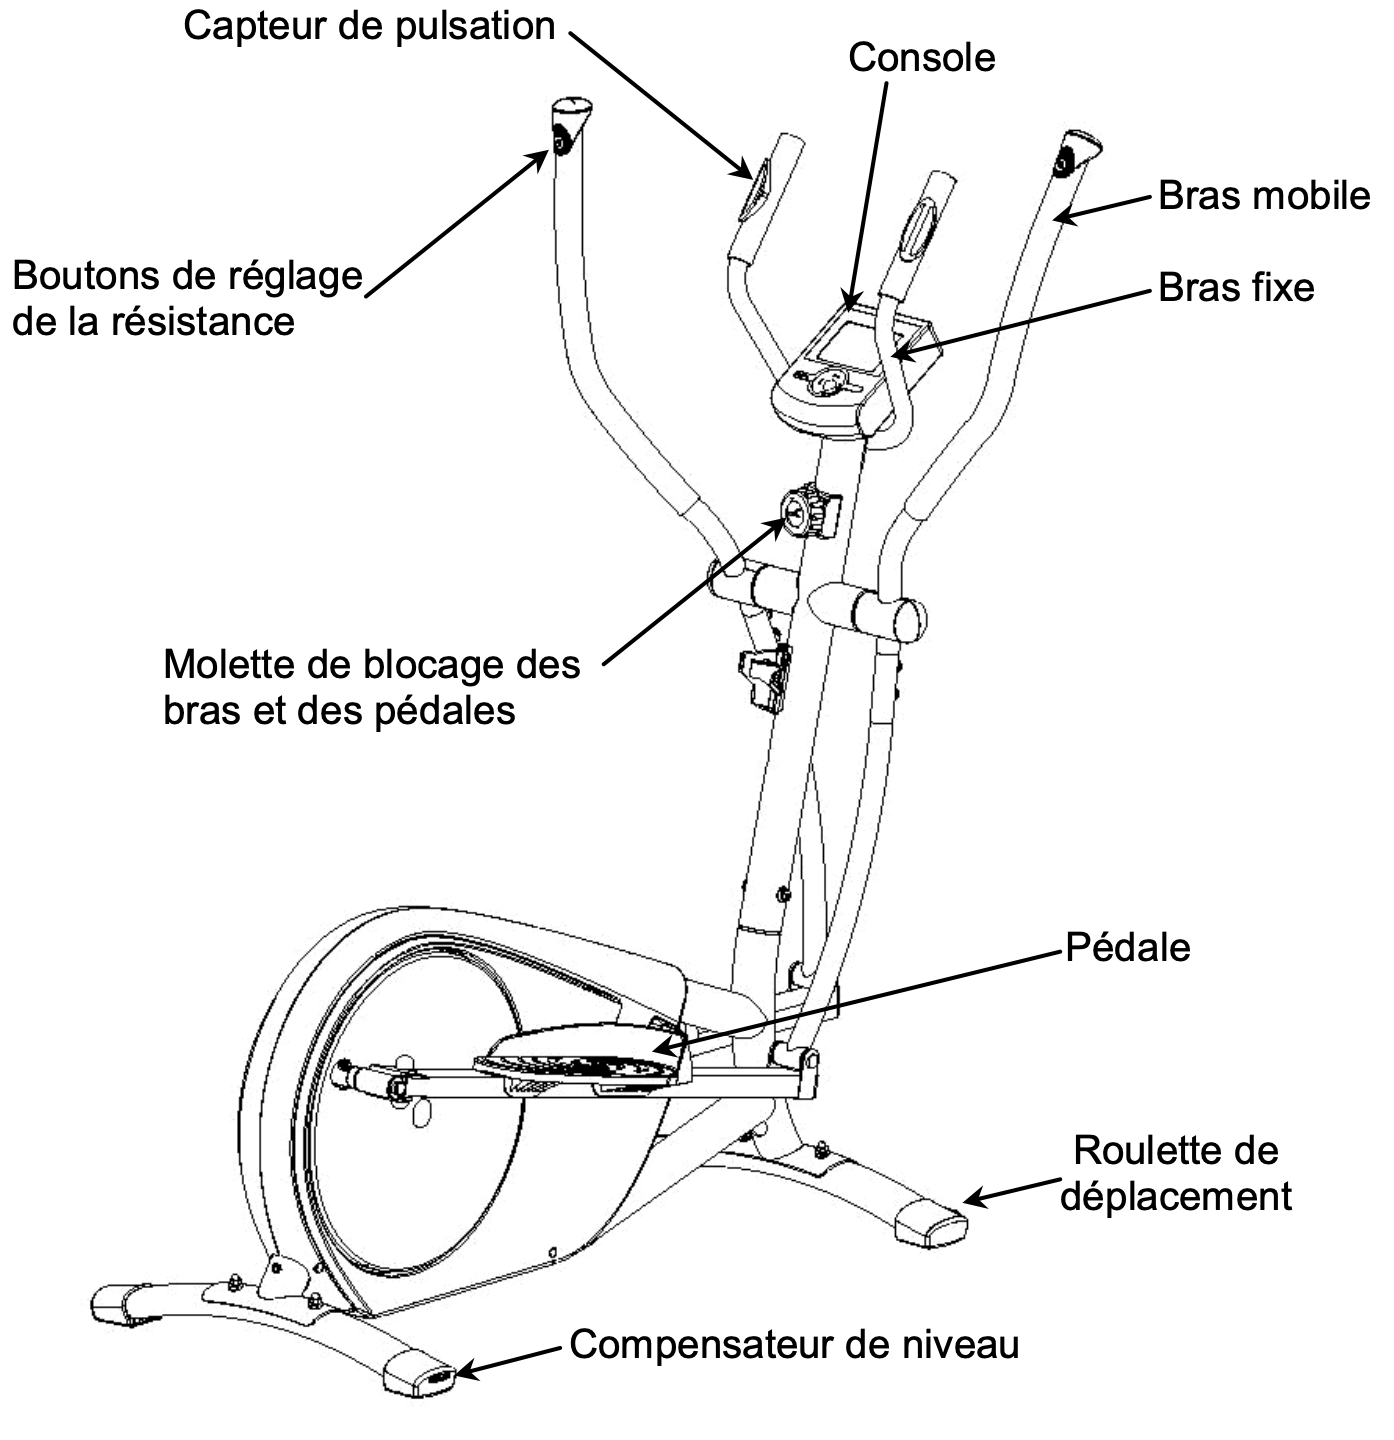
\includegraphics[width=1\textwidth,height=\textheight]{CM3/Velo-fonctionnelle-02.png}
\end{center}
\end{minipage}%

\end{figure}%
\end{block}
\end{frame}

\subsection{Example 2}\label{example-2}

\begin{frame}{Example 2}
\textbf{Modélisation cinématique d'une Vélo elliptique}
\end{frame}

\begin{frame}{Etapes}
\phantomsection\label{etapes-8}
\begin{enumerate}
\tightlist
\item
  Regroupement des pièces en ensembles solides
\item
  Élaboration du graphe des liaisons
\item
  Construction du schéma cinématique
\end{enumerate}
\end{frame}

\begin{frame}{Etapes}
\phantomsection\label{etapes-9}
\begin{enumerate}
\tightlist
\item
  \textbf{Regroupement des pièces en ensembles solides}
\item
  {Élaboration du graphe des liaisons}
\item
  {Construction du schéma cinématique}
\end{enumerate}

\begin{figure}

\begin{minipage}{0.70\linewidth}
🔎 On regroupe les pièces dans des ensembles (appelés classes
d'équivalence cinématique)✍️ Un nom (un numéro par exemple)🔵 Une
couleur\end{minipage}%
%
\begin{minipage}{0.30\linewidth}
⬛ 1 bâti 🟥 2 bras 🟩 2 pédales 🟦 2 articulations 🟨 1 pédalier
\end{minipage}%

\end{figure}%
\end{frame}

\begin{frame}{Etapes}
\phantomsection\label{etapes-10}
\begin{enumerate}
\tightlist
\item
  {Regroupement des pièces en ensembles solides}
\item
  \textbf{Élaboration du graphe des liaisons}
\item
  {Construction du schéma cinématique}
\end{enumerate}

\begin{figure}

\begin{minipage}{0.70\linewidth}
✓ Choix d'une base pour le solide de référence (bâti) ✓ Recherche des
contacts entre les solides ✓ Étude des liaisons entre les
solides\end{minipage}%

\end{figure}%
\end{frame}

\begin{frame}{Etapes}
\phantomsection\label{etapes-11}
\begin{enumerate}
\tightlist
\item
  {Regroupement des pièces en ensembles solides}
\item
  \textbf{Élaboration du graphe des liaisons}
\item
  {Construction du schéma cinématique}
\end{enumerate}

\begin{figure}

\begin{minipage}{0.80\linewidth}
Analyser pour \textbf{\emph{chaque laiaison}}✓ Surfaces en contact →
(plan/plan, sphère/cylindre, \ldots) ✓ Degrés de liberté ✓
Identification de composants\end{minipage}%

\end{figure}%
\end{frame}

\begin{frame}{Etapes}
\phantomsection\label{etapes-12}
\begin{enumerate}
\tightlist
\item
  {Regroupement des pièces en ensembles solides}
\item
  \textbf{Élaboration du graphe des liaisons}
\item
  {Construction du schéma cinématique}
\end{enumerate}

\begin{figure}

\begin{minipage}{0.80\linewidth}
Analyser pour \textbf{\emph{chaque laiaison}}\(L_{0-2}\) : Pivot d'axe
\((𝐴,\vec{z})\) \(L_{0-3}\) : Pivot d'axe \((𝐵,\vec{z})\) \(L_{2-1}\) :
Pivot d'axe \((𝐶,\vec{y})\) \(L_{1-4}\) : Pivot glissant d'axe
\((𝐴,\vec{y})\) \(L_{3-4}\) : Pivot d'axe \((E,\vec{z})\)\end{minipage}%

\end{figure}%
\end{frame}

\begin{frame}{Etapes}
\phantomsection\label{etapes-13}
\begin{enumerate}
\tightlist
\item
  {Regroupement des pièces en ensembles solides}
\item
  {Élaboration du graphe des liaisons}
\item
  \textbf{Construction du schéma cinématique}
\end{enumerate}

\begin{figure}

\begin{minipage}{0.80\linewidth}
✓ Tracé des éléments de situation des liaisons ✓ Dessin des symboles des
liaisons {✓ Simuler}\end{minipage}%

\end{figure}%
\end{frame}

\begin{frame}{Etapes}
\phantomsection\label{etapes-14}
\begin{enumerate}
\tightlist
\item
  {Regroupement des pièces en ensembles solides}
\item
  {Élaboration du graphe des liaisons}
\item
  \textbf{Construction du schéma cinématique}
\end{enumerate}

\begin{figure}

\begin{minipage}{0.80\linewidth}
{✓ Tracé des éléments de situation des liaisons} {✓ Dessin des symboles
des liaisons} ✓ Simuler\end{minipage}%

\end{figure}%
\end{frame}

\subsection{💻 Simuler pour mieux
comprendre.}\label{simuler-pour-mieux-comprendre.-1}

\begin{frame}{💻 Simuler pour mieux comprendre.}
\begin{figure}

\begin{minipage}{0.50\linewidth}
✓ Simuler par example:

\begin{itemize}
\tightlist
\item
  Vitesses
\end{itemize}

\end{minipage}%
%
\begin{minipage}{0.50\linewidth}

\end{minipage}%
\newline
\begin{minipage}{0.50\linewidth}

\end{minipage}%

\end{figure}%
\end{frame}

\subsection{Message clé de cette
séance}\label{message-cluxe9-de-cette-suxe9ance}

\subsection{Questions?}\label{questions}

\subsection{References.}\label{references.}



\end{document}
